%%%%%%%%%%%%%%%%%%%%%%%%%%%%%%%%%%%%%%%%%%%%%%%%%%%%%%%%%%%%%%%%%%%
%%
%% objective - CSCS small project proposal
%%
%%%%%%%%%%%%%%%%%%%%%%%%%%%%%%%%%%%%%%%%%%%%%%%%%%%%%%%%%%%%%%%%%%%



%\documentclass[a4paper,twocolumn]{article}
%\documentclass[a4paper,10pt]{article}
\documentclass[12pt]{report}

\usepackage[sort&compress,super]{natbib}
\usepackage[english]{babel}
\usepackage{amsmath}
\usepackage{graphicx}
\usepackage{caption}
\usepackage{subcaption}
%\usepackage{subfigure}                                %% for creating nested figures within figures
\usepackage{graphicx}
\usepackage{url}
\usepackage{array}
\usepackage{algorithm,algorithmic}
\usepackage{tikz}
\usepackage{url}  
\usetikzlibrary{arrows}
\usetikzlibrary{mindmap,trees}
\usepackage[overlay,absolute]{textpos}
%\usepackage[latin1]{inputenc}
\usepackage{wrapfig}
\usepackage{makeidx}
\usepackage{listings}
\usepackage{color}
\usepackage{xcolor}
\usepackage{enumitem}
\usepackage[normalem]{ulem}
\usepackage{mathtools}
\usepackage{lscape}
\usepackage{hyperref}


\DeclarePairedDelimiter{\ceil}{\lceil}{\rceil}
\DeclarePairedDelimiter{\floor}{\lfloor}{\rfloor}

% Rounded boxes functionality
\usepackage[framemethod=tikz]{mdframed}
\definecolor{mycolor}{rgb}{0.122, 0.435, 0.698}

\newmdenv[innerlinewidth=0.5pt, roundcorner=4pt,linecolor=mycolor, backgroundcolor=lightgray, innerleftmargin=4pt,
innerrightmargin=4pt,innertopmargin=2pt,innerbottommargin=2pt]{mybox}



%\usepackage[colorlinks,linkcolor=blue,anchorcolor=blue,citecolor=green]{hyperref} % hyper reference to contents 

\citestyle{plain}

\makeindex



% The following parameters seem to provide a reasonable page setup.
\topmargin 0.0cm
\oddsidemargin 0.2cm
\textwidth 16.1cm 
\textheight 21cm
\footskip 1.0cm



\begin{document}

\lstset{language=C++, breaklines=true}



\begin{titlepage}




\begin{center}
    
\noindent \textsc{{\Large Dune-CurvilinearGrid}}

\vspace{5mm}

\noindent \textbf{\textsc{{\Large Parallel grid for unstructured tetrahedral curvilinear meshes}}}
  
\vspace{2mm}
    
{\large
    
\noindent Aleksejs Fomins$^{\mathrm{a,b}}$ and Benedikt Oswald$^{\mathrm{b}}$

  }

\vspace{1mm}

\noindent $^{\mathrm{a}}$ Nanophotonics and Metrology Laboratory (\texttt{nam.epfl.ch})
\noindent Ecole Polytechnique F\'ederale de Lausanne (EPFL)
  
\vspace{1mm}

\noindent $^{\mathrm{b}}$ LSPR AG, Technopark Z\"urich, Technoparkstrasse 1, CH-8005 Z\"urich
\noindent phone +41 43 366 90 74 - email: \texttt{aleksejs.fomins@lspr.ch} and \texttt{benedikt.oswald@lspr.ch}

\vspace{2mm}

\end{center}



%%%%%%%%%%%%%%%%%%%%%%%%%%%%%%%%%%%%%%%%%%%%%%%%%%%%%%%%%%%%%%%%%%%%%%%%
% ACKNOWLEDGEMENTS
%%%%%%%%%%%%%%%%%%%%%%%%%%%%%%%%%%%%%%%%%%%%%%%%%%%%%%%%%%%%%%%%%%%%%%%%



\vspace{15mm}
\noindent \textbf{Acknowledgements} - While the architecture, implementation and down-to-earth programming
work for \texttt{dune-curvilineargrid} grid manager is credited with Aleksejs Fomins and Benedikt Oswald,
both of them are pleased to acknowledge the inspiration and support from the wider
\text{DUNE} community. We mention names in alphabetical order and sometimes associated with a specific
subject. In case we have forgotten to acknowledge an important contributor we kindly ask you to inform us and we will be
happy to insert the name immediately. So, then, here we are:
%%
%%
\textit{Peter Bastian}, Professor at University of Heidelberg, Germany
initial suggestion to consider curvilinear tetrahedral grids in order to reduce the computational burden onto the complex linear solver;
%%
%%
\textit{Markus Blatt}, Heidelberg, Germany, based independent high performance computing and \text{DUNE} contractor,
numerous hints related to the build system and \text{DUNE} architecture;
%%
%%
\textit{Andreas Dedner}, professor, University of Warwick, United Kingdom,
numerous hints related to the \text{DUNE} architecture;
%%
%%
\textit{Jorrit 'Hippi Joe' Fahlke}, postdoctoral scientist, University of M\"unster, Germany,
numerous hints related to the \text{DUNE} architecture, grid API, grid testing
and many other fields;
%%
%%
\textit{Dominic Kempf}, Phd student, University of Heidelberg, Germany
support w.r.t grid API implementation in \text{DUNE};
%%
%%
\textit{Robert Kloefkorn}, senior research scientist, IRISI, Norway,
support w.r.t grid API implementation in \text{DUNE};
%%
%%
\textit{Martin Nolte}, postdoctoral scientist, University of Freiburg im Breisgau, Germany,
numerous hints related to the \text{DUNE} architecture;
%%
%%
\textit{Oliver Sander}, professor, TU Aachen, Germany,
numerous hints related to the \text{DUNE} architecture,
numerical integration and quadrature;





%%%%%%%%%%%%%%%%%%%%%%%%%%%%%%%%%%%%%%%%%%%%%%%%%%%%%%%%%%%%%%%%%%%%%%%%
% BY WHOM DEVELOPMENT WAS SPONSORED
%%%%%%%%%%%%%%%%%%%%%%%%%%%%%%%%%%%%%%%%%%%%%%%%%%%%%%%%%%%%%%%%%%%%%%%%



\vspace{20mm}
{\small
\noindent \textbf{LEGAL NOTICE} - The development of the \texttt{dune-curvilineargrid} grid manager is sponsored by \textbf{LSPR AG},
Technopark Z\"urich, Technoparkstrasse 1, CH-8005 Z\"urich. \textbf{LSPR AG} exclusively holds all rights associated with \texttt{dune-curvilineargrid}.
%%
%%
The \texttt{dune-curvilineargrid} fully parallel grid manager will be made publicly available via \texttt{Github}
and free software based on the GPLv2 license. Other licenses can be negotiated through
\texttt{benedikt.oswald@lspr.ch}.
%%
%%
We herewith exclude any liability on the part of \textbf{LSPR AG} since the software is made available as is. Any user uses the software
at his own risk and by no means \textbf{LSPR AG} assumes any responsibility for harmful consequences or any other damage caused
by the use of the software. In particular, we emphasise that the whole project is governed by Swiss Law and nothing else.  Especially,
we reject any attempt of any other sovereign law to cover what we do.
}









\pagebreak

%%%%%%%%%%%%%%%%%%%%%%%%%%%%%%%%%%%%%%%%%%%%%%%%%%%%%%%%%%%%%%%%%%%%%%%%
% BEGIN OF ABSTRACT
%%%%%%%%%%%%%%%%%%%%%%%%%%%%%%%%%%%%%%%%%%%%%%%%%%%%%%%%%%%%%%%%%%%%%%%%

\vfill

\noindent \textbf{\textsc{ABSTRACT}} - We introduce the \texttt{dune-curvilineargrid} module. The module provides the self-contained, parallel
grid manager \texttt{dune-curvilineargrid} for curvilinear tetrahedral elements up to $5^{\mathrm{th}}$  order and conforms to the \text{DUNE} grid API.
%%
In particular, \texttt{dune-curvilineargrid} is a grid manager in its own right which offers this functionality:
%%
%%
\textbf{(1)} fully parallel mesh input in the \texttt{Gmsh} mesh format, thus we achieve the scalable input of very large meshes;
i.e. when a large mesh is read from disk, every process in the parallel context reads a small piece of the mesh; thus, we avoid the
scalability bottleneck that would arise if the whole mesh were read on the master process and then communicated to other processes;
the latter approach would inevitably lead to memory congestion on the master node and crash the program;
%%
%%
\textbf{(2)} once the mesh has been read from disk, it is partitioned using the \texttt{Parmetis} graph partitioning tool;
%%
%%
\textbf{(3)} \texttt{dune-curvilineargrid} manages meshes that consist of tetrahedra with curvilinear faces and edges, up to
$5^{\mathrm{th}}$ order; the curvilinear mesh geometry is modelled through \textit{Lagrange} polynomials of the respective order;
%%
%%
\textbf{(4)} since \texttt{dune-curvilineargrid} is a fully parallel grid manager for distributed memory architectures, it provides
globally unique indices over all processes in the parallel context.
%%
%%
\textbf{(5)} the \texttt{dune-curvilineargrid} fully parallel grid manager provides ghost elements associated with the interprocessor
boundaries;
%%
%%
\textbf{(5)} the \texttt{dune-curvilineargrid} grid manager provides communication protocols via the standard
\text{DUNE} data handle interface for all codimensions; i.e. data associated with vertices, edges, faces and volumes can
be communicated.
%%
%%
%%
%%
The \texttt{dune-curvilineargrid} grid manager is continously developed and improved. Among other things, we are working
on local refinement, modelling hanging nodes, non-uniform curvilinear order, periodicity and internal boundaries which
may become interesting for the implementation of hybrid finite-element-boundary-integral (FEBI) discretisation schemes.





%%%%%%%%%%%%%%%%%%%%%%%%%%%%%%%%%%%%%%%%%%%%%%%%%%%%%%%%%%%%%%%%%%%%%%%%
% END OF ABSTRACT
%%%%%%%%%%%%%%%%%%%%%%%%%%%%%%%%%%%%%%%%%%%%%%%%%%%%%%%%%%%%%%%%%%%%%%%%





\end{titlepage}


\tableofcontents





\chapter{Introduction}

%%%%%%%%%%%%%%%%%%%%%%%%%%%%%%%%%%%%%%%%%%%%%%%%%%%%%%%%%%%%%%%%%%%%%
% Curvilinear Grid Outline - Section on capabilities of the Grid
%%%%%%%%%%%%%%%%%%%%%%%%%%%%%%%%%%%%%%%%%%%%%%%%%%%%%%%%%%%%%%%%%%%%%

\section{Outline}
\subsection{Capabilities}

\noindent
Currently the curvilinear grid supports the following functionality.
\begin{itemize}
	\item Self-consistent grid manager supporting 3D tetrahedral curvilinear grids.
	\item GMSH input files of curvilinear orders 1-5. Usual linear geometries also supported
	\item Parallel mesh reader with scalability for large meshes and processors
	\item Mesh partitioning using ParMetis \textbf{CITE}
	\item Unique physical tag for each element and domain boundary. Read from GMSH file and accessible via grid methods.
	\item Unique global index for entities of all codimensions.
	\item Ghost elements of all codimensions (optional)
	\item Communication protocols for all codimensions
\end{itemize}

\noindent
The following functionality is currently NOT supported. As seen below, some of this functionality will be implemented in the nearest future, some other is not currently foreseen. We welcome contributions from the community
\begin{itemize}
	\item $[1-2 months]$ Location of containing element by global coordinate (via OCTree)
	\item $[1/2 year]$  Does NOT support global and local refinement
	\item $[1/2 year]$  Does NOT support hanging nodes
	\item $[1/2 year]$  Does NOT support periodic boundaries at the moment
	\item $[1 year]$    Does Not support curvilinear meshes of non-uniform order
	\item $[Undefined]$ Does NOT support 1D and 2D geometries. 
	\item $[Undefined]$ Does NOT support non-tetrahedral meshes.
	\item $[Undefined]$ Does NOT support front/overlap elements at the moment
\end{itemize}

\subsection{Design decisions}

\begin{itemize}
	\item User must provide globalId's for vertices and elements. [Automatically implemented by GMSH]
	\item User must provide all boundary segments inside GMSH file.
\end{itemize}


\subsection{Internal Structure}


Curvilinear Geometry:
\begin{itemize}
	\item Polynomial - Stores polynomials explicitly. Is able to perform basic arithmetic operations with polynomials, as well as differentiation and integration over a reference element.
	\item CurvilinearElementInterpolator
	\item CurvilinearGeometryHelper
	\item NumericalRecursiveInterpolationIntegrator
	\item CurvilinearGeometry
\end{itemize}

Curvilinear Grid
\begin{itemize}
	\item CurvilinearGMSHReader
	\item CurvilinearVTKWriter
	\item CurvilinearGridBase
		\subitem CurvilinearGridStorage
		\subitem CurvilinearGridConstructor
	\item CurvilinearGrid
	\item AllCommunicate
	\item VectorHelper	
	
\end{itemize}









\chapter{Usage}

%%%%%%%%%%%%%%%%%%%%%%%%%%%%%%%%%%%%%%%%%%%%%%%%%%%%%%%%%%%%%%%%%%%%%
% Curvilinear Grid Howto - Section on tutorials
%%%%%%%%%%%%%%%%%%%%%%%%%%%%%%%%%%%%%%%%%%%%%%%%%%%%%%%%%%%%%%%%%%%%%

\noindent
In order to start using the \curvgrid{} module we recommend to study the source code of the tutorials provided in \textit{curvilineargridhowto} folder. The tutorials use progressively more complicated concepts, so it is recommended to address them in the indexed order.


\subsection{Preliminaries - Creating Grid}
\label{usage-howto-tutorial-preliminaries}

All tutorials of \curvgrid{} reuse the simple auxiliary routine located in \textit{creategrid.hh}. This routine contains paths to all meshes currently used in tutorials, allowing the user to select the desired mesh by providing its index. It then proceeds to initialize the logging mechanisms
\begin{mybox}
\begin{lstlisting}
    Dune::LoggingMessage::init(mpihelper);
    Dune::LoggingTimer<Dune::LoggingMessage>::init(mpihelper);
\end{lstlisting}
\end{mybox}

\noindent
These singleton classes are essential for \curvgrid{}, as they support the parallel logging of the grid reading, construction and writing process, as well as later statistics on performance of individual routines. They can also be used by the user to write user logging output and time user functions, comparing them to the grid construction time. The next step is initializing the \textit{Curvilinear Grid Factory}

\begin{mybox}
\begin{lstlisting}
  Dune::CurvilinearGridFactory<GridType> factory(withGhostElements, withGmshElementIndex, mpihelper);
\end{lstlisting}
\end{mybox}

\noindent
where the boolean variable $withGhostElements$ determines whether the Ghost elements will be constructed and $withGmshElementIndex$ determines if the global element index from \gmsh{} is going to be reused by the grid (recommended). Otherwise, the index is automatically generated (see Tutorial 6 for discussion). After the above prerequisites, the curvilinear \gmsh{} reader is used to read the mesh file, partition it and write it to the provided grid factory.

\begin{mybox}
\begin{lstlisting}
  Dune::CurvilinearGmshReader< GridType >::read(factory, filename, mpihelper); 
\end{lstlisting}
\end{mybox}

\noindent
The \textit{Curvilinear Grid Factory} extends the interface of the standard dune grid factory, and therefore it will not work with other grids available in Dune. In order to achieve that, one must instead use the provided \textit{FactoryWrapper}. This wrapper class adheres to the standard grid factory interface, and disregards any process tag or curvilinear information provided by the curvilinear \gmsh{} reader. \\

\noindent
Finally, the grid is constructed, providing the user with the associated pointer. We note that the user must delete the grid pointer after use. %This is due to the fact that the factory used to create the grid ceases to exist before the grid itself.

\begin{mybox}
\begin{lstlisting}
  GridType *grid = factory.createGrid();
\end{lstlisting}
\end{mybox}

\subsection{Tutorial 1 - Getting started}
\label{usage-howto-tutorial-gettingstarted}

\noindent
This tutorial uses the above procedure to construct the \curvgrid{} by reading it from a \gmsh{} file. This and all other tutorials can be run both in serial and in parallel. First we define the grid

\begin{mybox}
\begin{lstlisting}
  typedef Dune::CurvilinearGrid<ctype, dim, isCached> GridType;
\end{lstlisting}
\end{mybox}

\noindent
where $dim=3$ is the dimension of the grid, $ctype=double$ is the underlying real type, and the $isCached$ is a boolean variable determining if the curvilinear geometry caching is used (recommended). Currently, only 3D tetrahedral grids are available. Then, the curvilinear grid is created by the $createGrid$ procedure described above. Finally, if we are interested in the time statistics for reading and construction of the grid, it can be obtained using the following command

\begin{mybox}
\begin{lstlisting}
  Dune::LoggingTimer<Dune::LoggingMessage>::reportParallel();
\end{lstlisting}
\end{mybox}



\subsection{Tutorial 2 - Traverse}
\label{usage-howto-tutorial-traverse}

This tutorial repeats the procedure from tutorial 1 to create the grid. It then iterates over the grid and extracts relevant information from the curvilinear entities. Currently, \curvgrid{} does not support refinement, so both leaf and level iterators will only iterate over the parent entities. As of \dune{} 2.4 revision the range-based for iterators introduced in \textit{c++11} standard are the preferred way to perform grid iteration. The below example iterator will iterate over all entities of the grid of a given codimension

\begin{mybox}
\begin{lstlisting}
  LeafGridView leafView = grid.leafGridView();
  for (auto&& elementThis : entities(leafView, Dune::Dim<dim - codim>())) {...}
\end{lstlisting}
\end{mybox}


Now, we would like to extract some relevant information from the iterator
\begin{mybox}
\begin{lstlisting}
  Dune::GeometryType gt = elementThis.type();
  LocalIndexType  localIndex
    = grid.leafIndexSet().index(elementThis);
  GlobalIndexType globalIndex
    = grid.template entityGlobalIndex<codim>(elementThis);
  PhysicalTagType physicalTag
    = grid.template entityPhysicalTag<codim>(elementThis);
  InterpolatoryOrderType interpOrder
    = grid.template entityInterpolationOrder<codim>(elementThis);
  BaseGeometry geom
    = grid.template entityBaseGeometry<codim>(elementThis);
  std::vector<GlobalCoordinate> interpVertices = geom.vertexSet()
\end{lstlisting}
\end{mybox}

\noindent
The $GeometryType$ and $LocalIndex$ are standard in \dune{}. $GlobalIndex$ provides a unique integer for each entity of a given codimension, over all processes. $PhysicalTag$ is the material tag associated with each entity, obtained from the mesh file. It can be used to relate to the material property of the entity, or to emphasize its belonging to a particular subdomain. In current \dunegrid{} standard this information can only be obtained by through the reader and requires auxiliary constructions. $InterpolatoryOrder$ denotes the integer polynomial interpolation order of the geometry of the entity. Currently, \curvgrid{} supports orders 1 to 5, the limiting factor being the curvilinear vertex indexing mapper in the reader. Finally, the $entityBaseGeometry$ gives the user direct access to the curvilinear geometry class of the entity, thus extending the interface provided by \textit{Dune::Grid::Geometry}. For example, it can be used to obtain the set of interpolatory vertices of the geometry, or an analytic polynomial matrix representing its Jacobian. \\






\subsection{Tutorial 3 - Visualization}
\label{usage-howto-tutorial-visualisation}

This tutorial demonstrates a simple way to output the curvilinear grid and associated vector fields (e.g. solutions of your PDE) to a PVTU file set using the \textit{CurvilinearVTKGridWriter} class. The writer is able to output arbitrary number of user-defined fields. The fields can be scalar or vector, and can be associated either with elements or with boundary faces. The sampled fields must overload the \textit{Dune::VTKScalarFunction} or \textit{Dune::VTKVectorFunction} standard provided by \curvgrid{}, and thus adhere to the following interface:

\begin{mybox}
\begin{lstlisting}
    // Writer initializes the functor once per each entity. This procedure can be used to pre-compute any quantities that do not change over the entity, accelerating the output
    virtual void init (const Entity & entity) {...}

    // Procedure that returns the field value as a function of local (!) coordinate
    virtual Range evaluate(const Domain & x) const  {...}

    // Procedure that returns the field name as it will appear in output file
    virtual std::string name() const  { return "localIndex2D"; }
\end{lstlisting}
\end{mybox}

\noindent
We provide 6 examples:
\begin{itemize}
  \item Element index scalar in 3D, written over all elements of the grid;
  \item Boundary segment index scalar in 2D, written over all boundary segments of the grid;
  \item Local sinusoidal vector in 3D, written over all elements of the grid;
  \item Local sinusoidal vector in 2D, written over all boundary segments of the grid;
  \item Global sinusoidal vector in 3D, written over all elements of the grid;
  \item Global sinusoidal vector in 2D, written over all boundary segments of the grid;
\end{itemize}

\noindent
These examples illustrate the important difference between local and global coordinates. Local coordinates are unique for each element, so one shall observe unique field behavior for each element. Global coordinates on the other hand are the same for all elements, thus providing a single continuous sinusoid across the entire mesh. The local fields are associated with the orientation of the element in space, which is arbitrary up to the permutation of element corners. Thus, to correctly display local fields, one must consider the orientation of the element. This can be achieved by considering the global coordinates and/or global indices of the corner vertices of the element, and of the intersection faces in between two elements. \\

\noindent
We start by constructing a curvilinear grid as previously demonstrated. We then proceed to initialize the writer, as well as fix its virtual refinement order to 15. We do this because we want to resolve the details of the sinusoid function to a very high precision, and because the mesh size is small. This operation is time-consuming, and, in general, the user should be aware of quadratic complexity of virtual refinement, and choose the refinement order that is necessary and sufficient. Should we choose to avoid specifying a fixed refinement order, the writer will calculate this order itself by considering the curvilinear order of the element. This works fine for most FEM applications, unless the basis order of the element is larger than its curvilinear order.

\begin{mybox}
\begin{lstlisting}    
  Dune::CurvilinearVTKGridWriter<GridType> writer(*grid);
    
  const int userDefinedVirtualRefinement = 15;
  writer.useFixedVirtualRefinement(userDefinedVirtualRefinement);
\end{lstlisting}
\end{mybox}

\noindent
We proceed to stack the pointers to the above field functors into 4 arrays, distinguished by vector/scalar and 2D/3D fields. We have decided to use dynamic polymorphism to implement this functionality. While this may be less efficient than other implementations, it allows writing fields produced by different functors by the very same compact routine.

\begin{mybox}
\begin{lstlisting}    
  std::vector<BaseVTKScalarFunction2D *> vtkFuncScalarSet2D_;
  std::vector<BaseVTKScalarFunction3D *> vtkFuncScalarSet3D_;
  std::vector<BaseVTKVectorFunction2D *> vtkFuncVectorSet2D_;
  std::vector<BaseVTKVectorFunction3D *> vtkFuncVectorSet3D_;

  vtkFuncScalarSet2D_.push_back(
    new VTKFunctionBoundarySegmentIndex<GridType>(*grid));
  vtkFuncScalarSet3D_.push_back(
    new VTKFunctionElementIndex<GridType>(*grid));

  vtkFuncVectorSet2D_.push_back(new VTKFunctionLocalSinusoidFace());
  vtkFuncVectorSet2D_.push_back(new VTKFunctionGlobalSinusoidFace());
  vtkFuncVectorSet3D_.push_back(new VTKFunctionLocalSinusoidElem());
  vtkFuncVectorSet3D_.push_back(new VTKFunctionGlobalSinusoidElem());

  writer.addFieldSet(vtkFuncScalarSet2D_);
  writer.addFieldSet(vtkFuncScalarSet3D_);
  writer.addFieldSet(vtkFuncVectorSet2D_);
  writer.addFieldSet(vtkFuncVectorSet3D_);
  writer.write("./", "tutorial-3-output"););
\end{lstlisting}
\end{mybox}
	
	
\begin{figure}[H]
	\begin{subfigure}[b]{0.45\textwidth} \hspace{4mm} 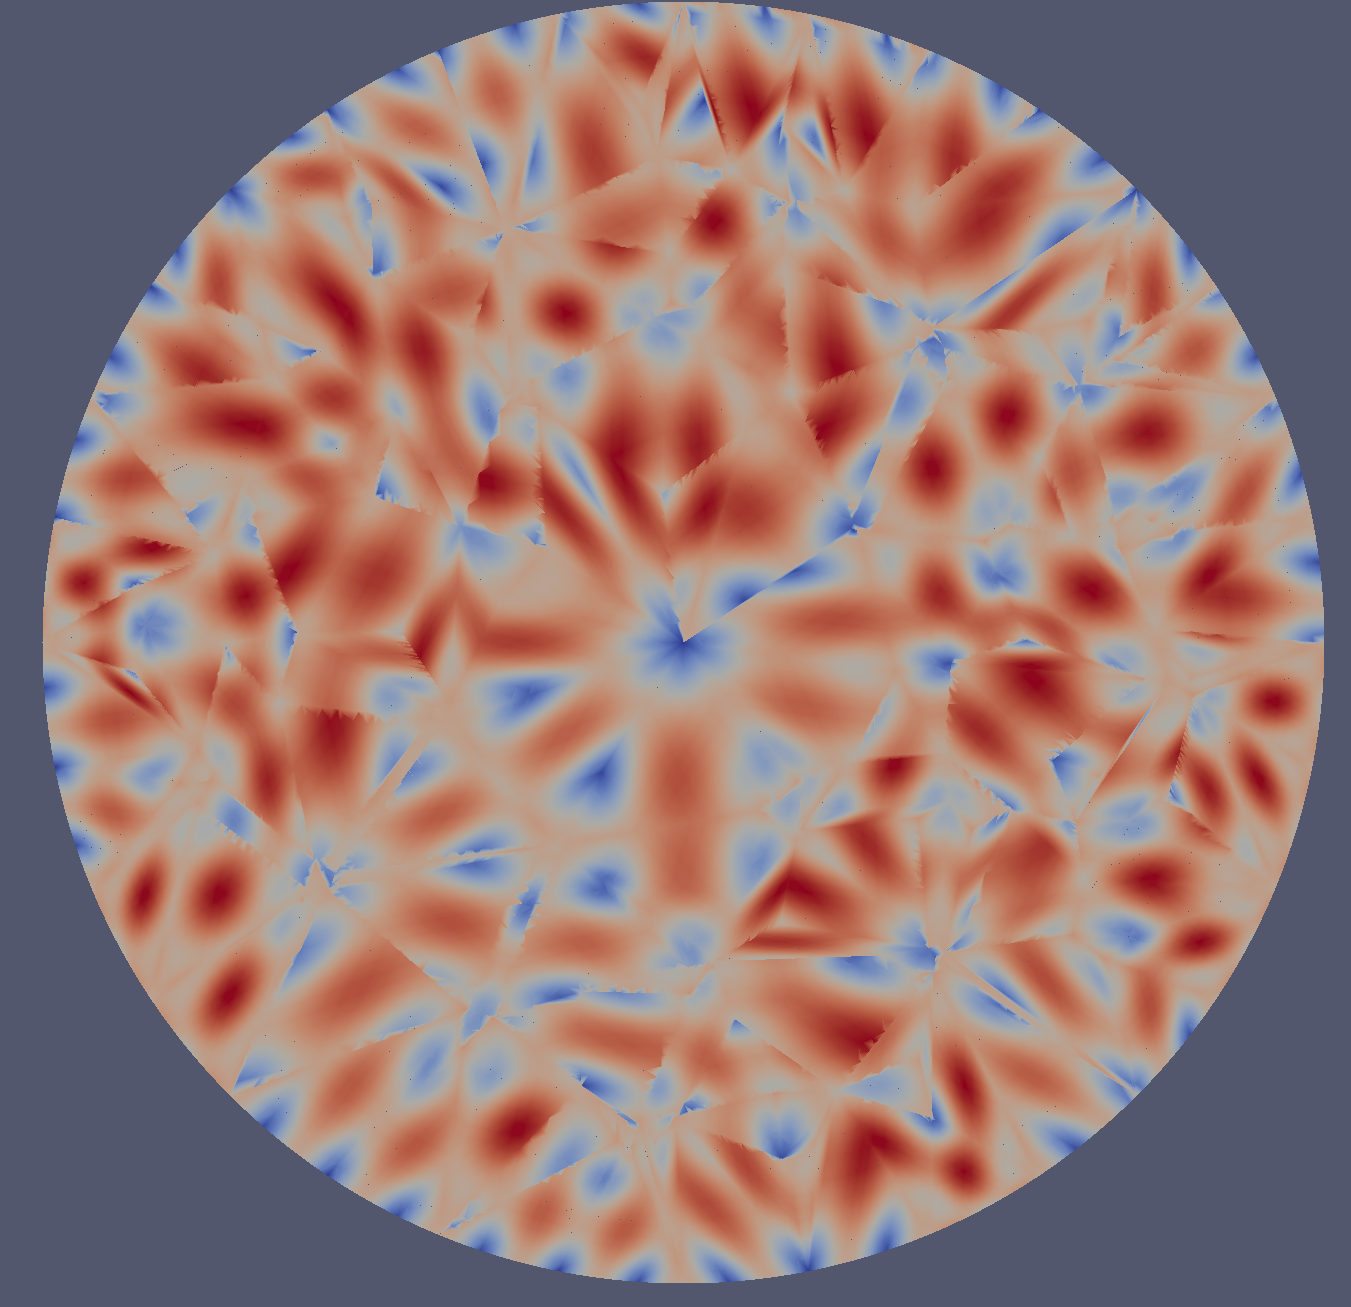
\includegraphics[scale=0.14]{images/tutorial3-vtk-localsinusoid} \end{subfigure}
	\begin{subfigure}[b]{0.45\textwidth} \hspace{4mm} 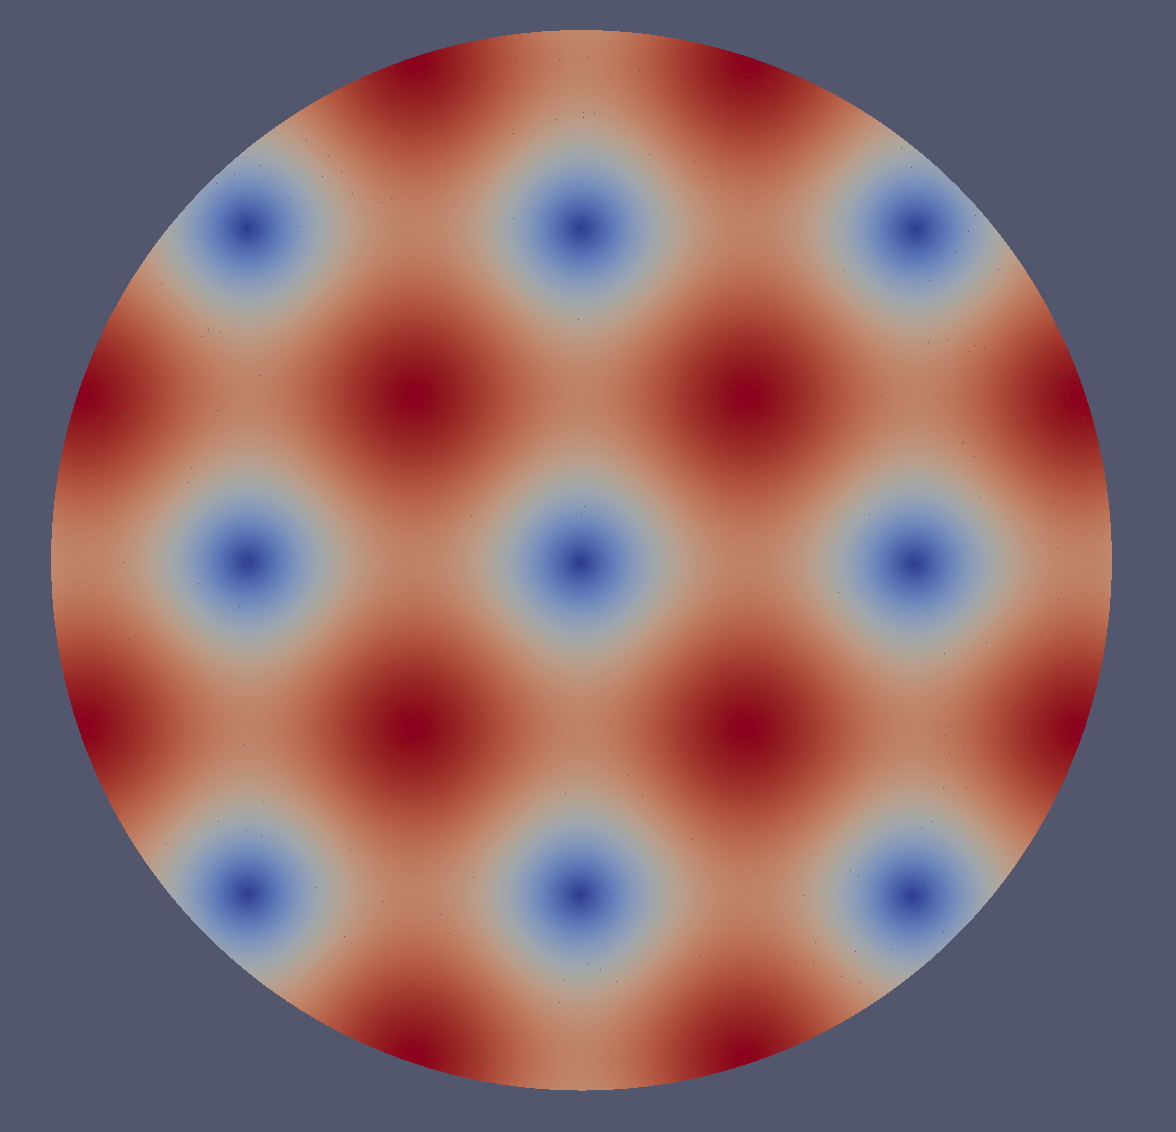
\includegraphics[scale=0.16]{images/tutorial3-vtk-globalsinusoid} \end{subfigure}
	\caption{ Visualization of tutorial 3. A sinusoid as function of local and global coordinates. This example emphasizes that there is no a priori orientation of the local coordinates. It is the task of the user to ensure that the local field is correctly oriented by considering the global indices of intersecting entities.}
	\label{fig:tutorial3:sinusoid}
\end{figure}


\subsection{Tutorial 4 - Quadrature Integration Tutorials}
\label{usage-howto-tutorial-integration-quadrature}

The following two tutorials demonstrate the capability of \curvgrid{} to address mathematical and physical problems requiring integration of certain quantities over the grid domain. \\


\noindent
\textbf{Scalar Surface Integral - \textit{Gauss} Law} \\
%
\noindent
In this example we verify \textit{Gauss} law numerically by computing the surface integral of the electric field produced by a unit point charge across the domain boundary of the mesh enclosing that charge. The tutorial will demonstrate that changing the curvature of the domain boundary or the position of the charge inside the domain does not affect the result that is $4 \pi$. More precisely, we compute the integral
\[\int_{\delta \Omega} \vec{E}(\vec{x}) \cdot d\vec{S} = \int_{\delta \Omega} \vec{E}(\vec{x}(\vec{u})) \cdot \vec{n}(\vec{u}) I(\vec{u}) d^2 u \]
\noindent
where $\vec{x}$ is the global coordinate, $\vec{u}$ is the coordinate local to the surface finite element,
\[\vec{E}(\vec{x}) = \frac{\vec{x} - \vec{x}_0}{|\vec{x} - \vec{x}_0|^{-3}}\]
is the electric field of a unit charge located at $\vec{x}_0$, $\vec{n}(\vec{u})$ is the surface outer normal in global coordinates as a function of local coordinates and
\[I(\vec{u}) = \sqrt{\det [ J^T(\vec{u}) J(\vec{u}) ]}\]
is the generalized integration element due to conversion of the integral from global to local coordinates (see \cref{appendix:integrationelements:proof}). \\

\noindent
In order to use the \curvgeom{} integration capabilities, the user must provide the integrand in the form of a functor class. The functor need not be overloaded, but must implement the $()$ operator

\begin{mybox}
\begin{lstlisting}
  ResultType operator()(const LocalCoordinate & x) const {...}
\end{lstlisting}
\end{mybox}

\noindent
as a function of the coordinate local to the entity it is evaluated over, in this case, a 2D coordinate local to a face. The code then iterates over all domain boundaries of the grid, calculating integrals of the functor over each boundary segment and adding up the results. In order to integrate a functor, the \textit{QuadratureIntegrator} class needs to be provided with the entity geometry, the functor to be integrated, the relative and absolute tolerances to be used for integration, as well as the norm type to be used for the case of multidimensional integration. 
\begin{mybox}
\begin{lstlisting}
  typedef Dune::QuadratureIntegrator<ct, DIM2D>  Integrator2DScalar;
  typedef typename Integrator2DScalar::template Traits<Integrand2D>::StatInfo  StatInfo;	
  StatInfo thisIntegralG = Integrator2DScalar::template integrateRecursive<FaceGeometry, Integrand2D, NORM_TYPE>(geometry, gaussf, RELATIVE_TOLERANCE, ACCURACY_GOAL);
\end{lstlisting}
\end{mybox}

\noindent
\textit{StatInfo} is the return data type of the \textit{QuadratureIntegrator}, which is a pair of the integral result and the quadrature order at which the desired relative accuracy was achieved. Note that the absolute accuracy \textit{ACCURACY\_GOAL} is used to determine if the integral is close enough to 0, as relative accuracy can not be used for this purpose due to division by 0. \\



\noindent
\textbf{Surface Vector Integral - Normal Integral} \\
%
\noindent
This test demonstrates the capability of \textit{QuadratureIntegrator} to integrate vector quantities. It tests the well-known identity, stating that the integral over the unit outer normal over a closed bounded domain is 0.

\begin{equation}
	\oiint_{\partial \Omega} n_x dS = \oiint_{\partial \Omega} \vec{e}_x \cdot \vec{n} dS = \iiint_{\Omega} \nabla \cdot \vec{e}_x dV = 0
\end{equation}

\noindent
The implementation of this test is almost identical to the \textit{Gauss} integral test above. The only difference is that \textit{Dune::FieldVector} is used as a functor output, and internally, instead of taking the dot product between the outer normal and the electric field, the normal itself is returned


%\subsection{Tutorial 4 - Recursive Numerical Integration}
%\label{usage-howto-tutorial-integration-recursive}


\subsection{Tutorial 5 - Communication via the DataHandle Interface}
\label{usage-howto-tutorial-communication}

This tutorial, consisting of two parts, serves as a simple use-case of interprocessor communication through grid entities, which is achieved via the \textit{DataHandle} interface. \\

\noindent
In the first tutorial we explicitly select all entities of the grid that are supposed to communicate for each available communication protocol, and communicate a dummy constant. The goal is to confirm that all the expected entities were communicated over, and all others were not. In the second tutorial, the global index of each entity is sent according to the specified communication protocol, and compared to the global index on the receiving side. It is demonstrated that these indices match for each communicating pair, and an exception is thrown should this not be the case. \\

% \noindent
% Briefly, the procedure communicateConstant iterates over all process process boundary intersections, and marks its neighbour entities, if they will be sending or receiving within the provided interface. Then the custom DataHandleConst is used to perform the communication. This data handle communicates one and the same constant to all entities it is requested. The important thing is that whenever gather or scatter methods are called, it checks if the requested entity was marked for sending or receiving, and throws an error if it is not. Finally, the main procedure checks that the total number of entities that have received the constant is equal to the number of entities marked for receiving.

\noindent
\curvgrid{} implements the \textit{DataHandle} communicators in accordance to the standard \dune{} interface, and its functionality does not exceed that envisioned by the standard interface. Since these tutorials are rather involved, and the standard mechanism is well-documented within the standard \dune{} reference, the detailed explanation of these two tutorials is beyond the scope of this paper. For further information, the user is referred to the \textit{Dune Grid Howto} documentation, found in \url{www.dune-project.org}



\subsection{Tutorial 6 - Parallel Data Output}

This tutorial demonstrates the use of a small utility \textit{ParallelDataWriter} designed for sorted parallel output of vectors. It explores the benefits of using the global element index provided by the mesh, for debugging of parallel numerical codes. The tutorial demonstrate that a quantity sampled over all elements of the grid and sorted by the element global index is independent of the number of processes used. Thus, the user can directly compare the output file, generated by runs with varying process count. \\

\noindent
\textit{Important Note: This tutorial only works if the mesh-provided global element index is re-used by the curvilinear \gmsh{} reader (default). If this is not the case, the automatically generated global index will depend on the number of processes and destroy the above symmetry.}

\noindent
This tutorial samples the volume of the elements. However, the interface of the \textit{ParallelDataWriter} extends to writing vectors of data for each element as well. One must first define the class

\begin{mybox}
\begin{lstlisting}
  <class Grid, class IndexType, class DataType>
  class ParallelDataWriter
\end{lstlisting}
\end{mybox}

\noindent
where \textit{IndexType} and \textit{DataType} are the data types of index and data arrays respectively. They can be any of the Plain Old Datatype (POD) classes, as long as their size is fixed over all processes for the communication purposes. One would then proceed to call the writer routine

\begin{mybox}
\begin{lstlisting}
  static void writeParallelData2File(std::string filename, std::vector<IndexType> & interiorElementGlobalIndex, std::vector<int> & interiorElementNDof, std::vector<DataType> & data, const Grid & grid)
\end{lstlisting}
\end{mybox}

\noindent
where \textit{interiorElementNDof} denotes the number of data entries per global index, and \textit{data} stores all data entries for all global indices in a contiguous 1D vector. \\


\subsection{Tutorial 7 - Global Boundary Communicator}

\noindent
This tutorial demonstrates the capabilities of \curvgrid{} to handle dense boundary communication problems, such as the Boundary Integral (BI) method. In the BI method, the global matrix or part of it correspond to pairwise coupling of every two faces on a given closed surface, providing a fully populated, i.e. dense, matrix. Each processor needs to obtain complete information of all faces on a given surface, collected over all processes.

\begin{mybox}
\begin{lstlisting}
  typedef Dune::CurvGrid::GlobalBoundaryContainer<GridType> BoundaryContainer;
  BoundaryContainer container(*grid, isDomainBoundary, volumeTag, surfaceTag);
\end{lstlisting}
\end{mybox}

\noindent
In case \textit{isDomainBoundary} is set to true, the \textit{BoundaryContainer} does not require the last two parameters. Otherwise, one must specify the surface tag of the interior surface, as well as the volume tag of elements either on the interior or the exterior of the surface, all one or the other. The unit outer normal for each face of the surface is determined as the unit outer normal of the associated element. Thus, if one provides the volume tag of the elements on the outside of the interior surface, one will always receive the inner unit normal at a later stage, and will have to multiply all of them by -1 in order to obtain the unit outer normal. The \textit{BoundaryContainer} does not contain the surfaces already located on this process, in order to save space.  \\

\noindent
In order to iterate over the \textit{BoundaryContainer}, we implement the accompanying \textit{BoundaryIterator}

\begin{mybox}
\begin{lstlisting}
  BoundaryIterator iter(container);
  while (!container.end()) {...}
\end{lstlisting}
\end{mybox}

\noindent
The boundary iterator re-implements most of the functionality of the standard Dune iterator, such as \textit{geometry()}, \textit{unitOuterNormal()}, \textit{indexInInside()}, \textit{geometryInInside()}, as well as some additional functionality compactified into the same iterator to save on communication complexity, such as 

\begin{mybox}
\begin{lstlisting}
  template <int codim>
  UInt globalIndex(UInt subIndexInFace) const {...}

  template <int codim>
  UInt globalIndexInParent(UInt subIndexInElem) const 

  UInt order() const { }

  BaseGeometryEdge geometryEdge(UInt subIndex) const {..}
\end{lstlisting}
\end{mybox}

\noindent
The tutorial performs several tests of the communicated boundary, such as the normal integral from Tutorial 4, calculation of total number of edges, as well as the complementarity of the global index of boundary surfaces located on this process, and on the \textit{BoundaryContainer}. \\




\subsection{Tutorial 8 - Interior Boundary}

The last tutorial extends the \textit{Gaussian} integral tutorial to interior boundaries, performing integrals for a set of charges inside and outside of the boundary. This is a simple test to verify if the interior boundary of the mesh forms a closed surface.


%%\subsection{Tutorial 5 - Polynomial Manipulation and Integration}
%%\label{usage-howto-tutorial-polynomial}
%%
%%
%%\subsection{Tutorial 7 - Point Location - OCTree}
%%\label{usage-howto-tutorial-octree}













%%%%%%%%%%%%%%%%%%%%%%%%%%%%%%%%%%%%%%%%%%%%%%%%%%%%%%%%%%%%%%%%%%%%%
% Curvilinear Grid Diagnostics - Section on mesh statistics and visualisation
%%%%%%%%%%%%%%%%%%%%%%%%%%%%%%%%%%%%%%%%%%%%%%%%%%%%%%%%%%%%%%%%%%%%%

\section{Diagnostics tools}
\subsection{Mesh statistics}
\subsection{Visualisation}









\chapter{Interface - Curvilinear Geometry}

%%%%%%%%%%%%%%%%%%%%%%%%%%%%%%%%%%%%%%%
% Implementation of Polynomial Class
%%%%%%%%%%%%%%%%%%%%%%%%%%%%%%%%%%%%%%%
\section{Polynomial Class}
\label{interface-geometry-polynomial}


\noindent
Arbitrary polynomial of order up to $n$ with $d$ parameters can be represented in its expanded form as
\[ p(\vec{u}) = \sum_i A_i \prod_{j = 0}^d u_j^{\mathrm{pow}_{i,j}},  \]
for example in 3D this can be written as
\[ p(\vec{u}) = \sum_i A_i u^{pow_{u,i}} v^{pow_{v,i}} w^{pow_{w, i}},  \]

\noindent
Therefore, we define a Monomial class, which stores a constant multiplier $A$ and powers vector $pow$. \\

\begin{mybox}
\begin{lstlisting}
  PolynomialTraits::Monomial(double prefNew, std::vector<int> powerNew)
  PolynomialTraits::Monomial(double prefNew, int x)
  PolynomialTraits::Monomial(double prefNew, int x, int y)
  PolynomialTraits::Monomial(double prefNew, int x, int y, int z)
\end{lstlisting}
\end{mybox}




\subsection{Methods}
\label{interface-geometry-polynomial-methods}


A polynomial can be constructed either empty, from a single monomial or from a vector of monomials. \\

\begin{mybox}
\begin{lstlisting}
  Polynomial()
  Polynomial(Monomial M)
  Polynomial(std::vector<Monomial> Mvec)
\end{lstlisting}
\end{mybox}

\noindent
The below interface provides methods to perform basic algebraic operations with polynomials and scalars. The method $axpy$ is the scaled addition, equivalent to $this += other * a$ \\

\begin{mybox}
\begin{lstlisting}
  LocalPolynomial & operator+=(const Monomial & otherM)
  LocalPolynomial & operator+=(const LocalPolynomial & other)
  LocalPolynomial & operator*=(const double c)  
  LocalPolynomial & operator*=(const LocalPolynomial & other)  
  void axpy(LocalPolynomial other, double c)
  LocalPolynomial operator+(const LocalPolynomial & other)
  LocalPolynomial operator+(const ctype a)  
  LocalPolynomial operator-(const LocalPolynomial & other)  
  LocalPolynomial operator-(const ctype a)  
  LocalPolynomial operator*(const ctype a)  
  LocalPolynomial operator*(const LocalPolynomial & other)
\end{lstlisting}
\end{mybox}

\noindent
It is possible to differentiate, integrate and evaluate a polynomial. $derivative$ returns the partial derivative of the polynomial wrt coordinate indexed by the parameter. $evaluate$ evaluates the polynomial at the provided local coordinate. $integrateRefSimplex$ integrates the polynomial over the reference simplex of the same dimension as the polynomial, thus returning a scalar. An integral of a monomial over reference simplex has analytical expression, see the proof in appendix \ref{appendix-proof-simplexintegral}  \\


\begin{mybox}
\begin{lstlisting}
  LocalPolynomial derivative(int iDim)
  double evaluate(const LocalCoordinate & point)
  double integrateRefSimplex()
\end{lstlisting}
\end{mybox}


\noindent
The following auxiliary methods can be used to extract additional information about a polynomial. $order$ returns the largest power among all monomials, that is, the sum of powers of that monomial. Magnitude returns the largest absolute value prefactor over all monomials. $to\_string$ converts the polynomial to a string for further text output \\

\begin{mybox}
\begin{lstlisting}
  unsigned int order()
  double magnitude()
  std::string to_string()
\end{lstlisting}
\end{mybox}


\noindent
\uline{Compactify}: adds up all summands with the same power. Sorts the summands by $(x_1,y_1,z_1) < (x_2, y_2, z_2)$, where $x$ has the highest priority and $z$ has the lowest priority. Then all of the repeating powers will be consecutive. Simply loop over sorted polynomial, and to a new polynomial add the sums of all consecutive repeating polynomials.



\subsection{Tests}


\noindent
Currently the tests are only for 1, 2 and 3 dimensions. Most of the tests use intrinsic functionality like polynomial operators and derivatives to construct polynomials and print them to the screen, and request the user to to verify manually if they match the expected polynomials which are also printed. For each dimension there is one test which integrates a non-linear polynomial over simplex and prints out the result which is also compared manually. \\

\textbf{TODO:} These tests can and should be automatized in the future using integer string comparison. The test program should throw an error if a test fails

\section{CurvilinearGeometryHelper}


%%%%%%%%%%%%%%%%%%%%%%%%%%%%%%%%%%%%%%%
% Implementation of Interpolator Class
%%%%%%%%%%%%%%%%%%%%%%%%%%%%%%%%%%%%%%%
\section{Polynomial Interpolator Class}

\subsection{Methods}

\begin{itemize}
	\item \uline{Initialization:} Requires reference element/GeometryType, interpolatory vertex vector and interpolation order
	\item \uline{dofPerOrder:} Number of interpolatory vertices required for a given element type, dimension and interpolation order. For a simplex this quantity is
	\[ {DoF}_{dim}^{ord} = \{ \{ 2,3,4,5,6 \}, \{ 3,6,10,15,21 \}, \{ 4,10,20,35,56 \} \} \]
	\item \uline{cornerID:} The id number of a corner in the interpolatory vertex vector. For the simplices is calculated as follows:
		\subitem -for edge $\{ 0, \; ord \}$
		\subitem -for triangle $\{0, \; ord, \; {DoF}_{dim}^{ord} - 1\}$
		\subitem -for tetrahedron $\{0, \; ord, \; ord (ord + 3) / 2, \; {DoF}_{dim}^{ord} - 1\}$
	\item \uline{simplexGrid:} These 3 methods implement the functionality discussed in section \ref{subsection-simplexgrid}. They return a vector of indices which the grid points take in the d-dimensional matrix, and that vector divided by the interpolation order, which is exactly the local coordinates of the reference simplex grid.
	\item \uline{lagrangePolynomial:} Evaluates the i-th Lagrange Polynomial $L_i(\vec{r})$ for a given $i$ and a given local coordinate. Lagrange polynomials in this case are given explicitly for all orders to accellerate computation.
	\item \uline{realCoordinate:} Evaluates the global coordinate given a local coordinate. Computes the scalar product $\vec{p}(\vec{r}) = \sum_i \vec{p}_i L_i (\vec{r})$.
	\item \uline{interpolatoryVectorAnalytical:} Produces an analytical map from local to global coordinates in terms of polynomial vector.
		\subitem 0) Constructs local grid points $\vec{r}_i$ as given in \ref{subsection-simplexgrid}.		
		\subitem 1) Constructs monomial basis $\vec{z}^{ord}(\vec{r})$ as given in the beginning of section \ref{section-interppoly}
		\subitem 2) Evaluates all monomials $\vec{z}^{ord}(\vec{r})$ at all local grid points $\vec{r}_i$, assembling the DynamicMatrix V
		\subitem 3) Computes all lagrange polynomials using $\vec{L}(\vec{r}) = V^{-1} \vec{z}^{ord}(\vec{r})$
		\subitem 4) Computes the analytical map $\vec{p}(\vec{r}) = \sum_i \vec{p}_i L_i (\vec{r})$.
	\item \uline{SubentityInterpolators} Constructs Interpolator classes for each $\dim - 1$ subentity of the given element. Only allowed for elements of dimensions 2 and 3.
		\subitem - At the moment a rather crude algorithm is employed. To find the vertices corresponding to a given boundary, the order numbers of simplexGrid are written in a $(ord + 1) \times (ord + 1) \times (ord + 1)$ matrix, which is then used to easier locate the indices of the boundary interpolatory points in the vertex vector.
		\subitem - Certain orientation convention is chosen for the provided sub-entitiy interpolators, to simplify the future calculation of the outwards normals. The convention for edge orientations for a triangle $(012)$ are $(01)$, $(12)$ and $(20)$. The convention for triangle orientations for a tetrahedron $(0123)$ are $(012)$, $(023)$, $(213)$ and $(031)$.
\end{itemize}

\begin{figure}[hp]
    \centering
    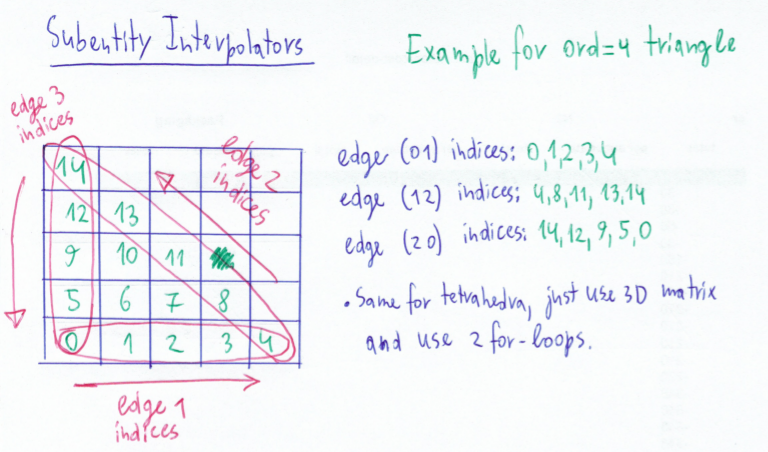
\includegraphics[scale=0.5]{doc-pics/pic-subentity-interpolators-method.png}
    %\caption{Awesome Image}
    %\label{fig:awesome_image}
\end{figure}


\subsection{Tests}

\noindent
For each dimension several linear and polynomial Functors are defined which act as pre-defined local-to-global maps. Then, for a simplex of each dimension there is a testing routine which is run for every applicable Functor. The tests are as follows:
\begin{itemize}
	\item For each order generate a local grid and sample the given functor to obtain global coordinates for interpolation points and thus construct the interpolator.
	\item First test requests a global coordinate for each local grid point, both using explicit function $realCoordinate$ and by evaluating the analytical polynomial provided by $interpolatoryVectorAnalytical$. Then the 3 results are compared. For this test, all 3 results must match independent of Functor and interpolation order.
	\item Second test requests a global coordinate for a random set of local coordinates, also comparing the correct result with explicit and analytical functionality. Explicit and analytical results should be equal to each other for any test since they do the same thing. However, they will match to the true result only if the polynomial order of the Functor is lower or equal to the one being tested, and most likely should fail for lower orders.
\end{itemize}

\textbf{TODO:}
\begin{itemize}
	\item The tests must be automatized such that the program throws an error if a test fails.
	\item Would be useful to test the method $SubentityInterpolators$ which is not tested at the moment, but is indirectly tested later in the LagrangeGeometry tests.
\end{itemize}


%%%%%%%%%%%%%%%%%%%%%%%%%%%%%%%%%%%%%%%
% Implementation of Recursive Integration
%%%%%%%%%%%%%%%%%%%%%%%%%%%%%%%%%%%%%%%
\section{Recursive Integrator Class}

Evaluates integral over element, approximating the integrand by an interpolatory polymomials of two hierarchical orders (2 and 4 at the moment). The running integration error is approximated by the difference between the analytical integrals calculated from these two interpolatory polynomials. The higher order element is split into into sub-elements of lower order, and the integration proceeds recursively. Every time an element is split, its previous running error is subtracted from the total error, and the running errors of the sub-elements are added to the total error. Thus, the integration is terminated when total approximated error is below selected tolerance. Heap structure ordered by the approximate error of the element is used to avoid recursion. At every iteration the element with the worst error is selected and then refined. When splitting, the previously calculated points are not re-calculated but hierarchically re-used by sub-elements. The sub-element only needs to be refined to a higher hierarchical order, by adding more points. \\

\noindent
\textit{Possible improvement - Performance}. As the the refined element does not check if the neighboring elements are also being refined, so they both sample on the boundary twice. Does there exist a method to store/find intersection refinements faster than just compute 2nd time. Using order 4 for every new refined triangle we sample 9 new points, out of which 2 are being wasted, thus $22\%$ inefficient.

\begin{figure}[p]
    \centering
    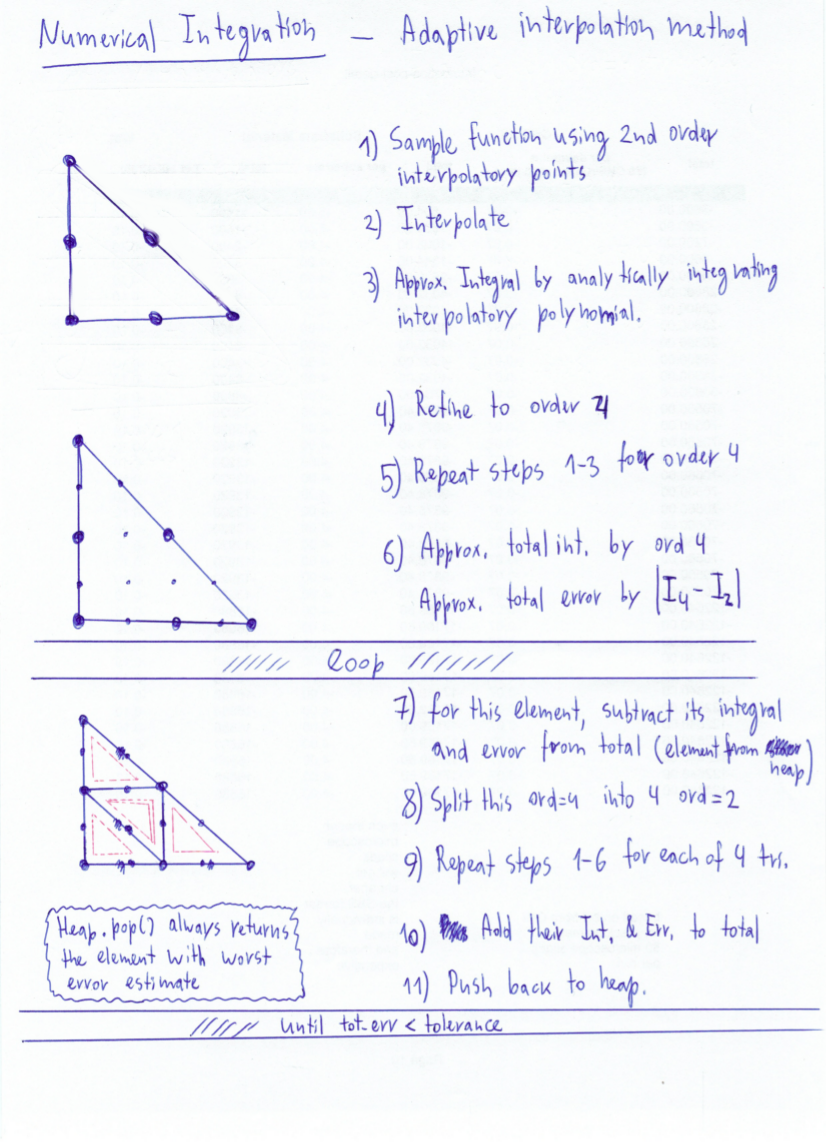
\includegraphics[scale=0.8]{doc-pics/pic-numerical-integration-adaptive-interpolation.png}
    %\caption{Awesome Image}
    %\label{fig:awesome_image}
\end{figure}


\subsection{Methods}

\noindent
Numerical Integration is only available for Simplices at the moment.

\noindent
\begin{itemize}
	\item \uline{Initialization:} Requires GeometryType to know the type of the element being integrated
	\item \uline{Integrate:} Integrates a function given by a functor object, until the expected integration error is below given tolerance.
\end{itemize}


\subsection{Tests}

\noindent
Numerical Integration is only implemented and hence tested for edges and triangles. A multitude of integrands are given in terms of Functors, starting with simple polynomial integrands and ending with integrands involving square roots of polynomials, as this is these are functions the method is expected to integrate well. The integrals are computed and compared to expected ones, which are sometimes given explicitly in numerical form, except of a lucky integral of $\iint \sqrt{xy} \; dxdy$ which happens to be $\pi / 24$. \\

\textbf{TODO:}
\begin{itemize}
	\item These tests should be automatized, which is easy to do, as they are only comparing numerical values.
	\item Integrals of complicated functions may exceed 100000 samples for this method given relative precision $10^{-5}$, which is too slow for the desired application
\end{itemize}


%%%%%%%%%%%%%%%%%%%%%%%%%%%%%%%%%%%%%%%
% Implementation of Curvilinear Geometry
%%%%%%%%%%%%%%%%%%%%%%%%%%%%%%%%%%%%%%%
\subsection{Curvilinear Geometry Base Class}
\label{interface-curvilineargeometry}

\noindent
Curvilinear Geometry can be initialized either using the interpolator class, or the parameters necessary to initialize the interpolator class \\

\begin{mybox}
\begin{lstlisting}
  CurvilinearGeometry ( const ElementInterpolator & elemInterp)
  CurvilinearGeometry ( const ReferenceElement &refElement, const Vertices &vertices, InterpolatoryOrderType order)
  CurvilinearGeometry ( Dune::GeometryType gt, const Vertices &vertices, InterpolatoryOrderType order)
\end{lstlisting}
\end{mybox}

\noindent
Standard dune functionality \\
\begin{mybox}
\begin{lstlisting}
  bool affine ()
  GlobalCoordinate center ()
\end{lstlisting}
\end{mybox}

\noindent
Wrapper for basic interpolator functionality \\
\begin{mybox}
\begin{lstlisting}
  InterpolatoryOrderType order()
  Dune::GeometryType type()
  int nCorner ()
  int nVertex ()
  GlobalCoordinate corner ( InternalIndexType cornerLinearIndex )
  GlobalCoordinate vertex (int i)
  std::vector< GlobalCoordinate > cornerSet()
  std::vector<GlobalCoordinate> vertexSet()
\end{lstlisting}
\end{mybox}

\noindent
Wrapper for extended interpolator functionality \\
\begin{mybox}
\begin{lstlisting}
  ElementInterpolator interpolator()
  PolynomialVector interpolatoryVectorAnalytical()

  template<int subdim>
  CurvilinearGeometry< ctype, subdim, cdim>  subentityGeometry(InternalIndexType subentityIndex)
\end{lstlisting}
\end{mybox}

\noindent
Mappings \\
\begin{mybox}
\begin{lstlisting}
  GlobalCoordinate global ( const LocalCoordinate &local )
  bool local ( const GlobalCoordinate &globalC, LocalCoordinate & localC )
\end{lstlisting}
\end{mybox}

\noindent
Construction of normals \\
\begin{mybox}
\begin{lstlisting}
  GlobalCoordinate normal(const LocalCoordinate &local )
  GlobalCoordinate subentityNormal(InternalIndexType indexInInside, const LocalCoordinate &local )
  GlobalCoordinate subentityUnitNormal(InternalIndexType indexInInside, const LocalCoordinate &local )
  GlobalCoordinate subentityIntegrationNormal(InternalIndexType indexInInside, const LocalCoordinate &local )
\end{lstlisting}
\end{mybox}

%\noindent
%Construction numerical and analytic integration elements. \\

%\noindent
%\uline{JacobianDeterminantAnalytical}: $|\det J_{ij}|$ is available explicitly in polynomial form, when $(dim_{elem} = dim_{world})$. Although modulus is not a polynomial operation, $\det J_{ij} \neq 0$ inside the element, because the geometry must not be self-intersecting. Hence $\det J_{ij}$ is not allowed to change sign within the element, and modulus-correction is to evaluate $\det J_{ij}$ anywhere inside the element and multiply the analytic expression by $-1$ if the result is negative. \\

%\noindent
%\uline{NormalIntegrationElementAnalytical}: Surface normal integration element $d\vec{S} = \vec{n} dS $ is available. For edges in 2D defined by $d\vec{l} = (\partial_u p_y, -\partial_u p_x) du$. For triangles in 3D defined by $d \vec{S} = -(\partial_u \vec{p} \times \partial_v \vec{p}) du dv $ \\

%\noindent
%\uline{IntegrationElementSquaredAnalytical}: The square of the pseudodeterminant $\det(JJ^T)$, when $(dim_{elem} \neq dim_{world})$. For edges this expression is equal to $|\partial_u \vec{p}|^2$. For triangles in 3D this expression is equal to $|\vec{dS} / (du \; dv)|^2$. \\



\noindent
Numeric integration provided via standard integration elements, that can be further used in a quadrature routine. An exception to the interface is the volume method, which has do be done recursively, since the integration element need not be polynomial. Here, CurvilinearGeometry directly uses the recursive quadrature, and thus requires a tolerance parameter to terminate.

\begin{mybox}
\begin{lstlisting}
  ctype integrationElement ( const LocalCoordinate &local )
  JacobianTransposed jacobianTransposed ( const LocalCoordinate &local )
  JacobianInverseTransposed jacobianInverseTransposed ( const LocalCoordinate &local )
  ctype volume (double tolerance)
\end{lstlisting}
\end{mybox}




%\subsubsection{Methods - Cached Lagrange Geometry}
%\label{interface-curvilineargeometry-cached-methods}



\subsubsection{Tests}

\noindent
We start by explicitly defining the local-global mapping functors to mimic LagrangeGeometry for simplices of all 3 dimensions (Table 2). Then the following test procedure is run for each of the simplex mapping:
\begin{itemize}
	\item Loop over 5 interpolatory orders.
	\item For each order sample the interpolatory points from the mapping. Construct LagrangeGeometry and CurvilinearLagrangeGeometry classes.
	\item \textbf{Test 1}. To test if the Geometry has been correctly initialized, return all of its corners and check if they match those evaluated by the function.
	\item \textbf{Test 2}. To test local-to-global functionality, a random set of local points is sampled over the element, and the result of method $global()$ of the Geometry is compared with that of the explicit mapping. The test is omitted if the interpolation order is smaller than the order of the mapping.
	\item \textbf{Test 3}. To test global-to-local functionality, the local method is used for all the interpolation points expecting to obtain the points of the local interpolation grid over reference simplex. Also, it is checked if all these points are reported to be inside the element. This test fails a lot:
		\subitem -Fails to consider the point that is close to the boundary as in.
		\subitem -Fails to converge to a boundary point if the geometry has a zero derivative on the corner or on the whole boundary.
	\item \textbf{Test 4}. To test global-to-local using more probable sample points, the local coordinates are randomly sampled. It is then verified if $\vec{p} \approx local(global(\vec{p}))$. This test also checks if all the sample points are reported inside as they should be.
	\item \textbf{Test 5}. To check if the outside points are correctly sampled outside, as well as check the correctness of surface normal, we loop over all boundaries of the element, construct boundary normals for a uniform grid on the each boundary, and obtain the points which are just outside the element by calculating $\vec{p} = \vec{g} + \alpha \vec{n}$, where $\vec{g}$ is the global coordinate of of some point on the boundary, $\vec{n}$ is the normal at that point, and $\alpha = 0.01$ is a small number. \cref{fig:geometry:test:normal}.
	\item \textbf{Test 6}. The scalar basis functions given in Table 1 are integrated over the Geometry, and results are compared to those calculated by hand, given in Table 2.
	\item \textbf{Test 7}. The dot product surface integrals of vector basis functions (given in Table 3) over the Geometry are compared to those calculated by hand, given in Table 4.
\end{itemize}

\begin{figure}
    \centering
    
\includegraphics[scale=1.0]{images/normaltest}
	\captionsetup{width=0.8\textwidth} 
	\caption{ A combined test for normal accuracy and ability to accurately determine that a vertex is outside the element. Face normals sampled over a grid are used to produce global coordinates just outside the the element, which are then checked for having a local coordinate inside that element. }
	\label{fig:geometry:test:normal}
\end{figure}

\subsubsection{Integral-tests}

\begin{center}
\begin{tabular}{ | l | l | l |}
  \hline
  Ord & Dim & Scalar Basis Function \\ \hline
  0 & 1 & $1$ \\ \hline
  1 & 1 & $1 + 2x$ \\ \hline
  2 & 1 & $1 + 2x + 3x^2$ \\ \hline
  3 & 1 & $1 + 2x + 3x^2 + 4x^3$ \\ \hline
  4 & 1 & $1 + 2x + 3x^2 + 4x^3 + 5x^4$ \\ \hline
  5 & 1 & $1 + 2x + 3x^2 + 4x^3 + 5x^4 + 6x^5$ \\ \hline
%%  
  0 & 2 & $1$ \\ \hline
  1 & 2 & $1 + 2(x + y)$ \\ \hline
  2 & 2 & $1 + 2(x + y) + 3(x^2 + y^2) + xy$ \\ \hline
  3 & 2 & $1 + 2(x + y) + 3(x^2 + y^2) + xy + 4(x^3 + y^3) + xy^2$ \\ \hline
  4 & 2 & $\begin{array}{lcl} 1 & + & 2(x + y) + 3(x^2 + y^2) + xy + 4(x^3 + y^3) + xy^2 \\ & + & 5(x^4 + y^4) + xy^3 \end{array}$ \\ \hline
  5 & 2 & $\begin{array}{lcl} 1 & + & 2(x + y) + 3(x^2 + y^2) + xy + 4(x^3 + y^3) + xy^2 \\ & + & 5(x^4 + y^4) + xy^3 + 6(x^5 + y^5) + xy^4 \end{array}$ \\ \hline
%%  
  0 & 3 & $1$ \\ \hline
  1 & 3 & $1 + 2(x + y + z)$ \\ \hline
  2 & 3 & $1 + 2(x + y + z) + 3(x^2 + y^2 + z^2) + xy$ \\ \hline
  3 & 3 & $1 + 2(x + y + z) + 3(x^2 + y^2 + z^2) + xy + 4(x^3 + y^3 + z^3) + xyz$ \\ \hline
  4 & 3 & $\begin{array}{lcl} 1 & + & 2(x + y + z) + 3(x^2 + y^2 + z^2) + xy + 4(x^3 + y^3 + z^3) + xyz \\ & + & 5(x^4 + y^4 + z^4) + xyz^2 \end{array}$ \\ \hline
  5 & 3 & $\begin{array}{lcl} 1 & + & 2(x + y + z) + 3(x^2 + y^2 + z^2) + xy + 4(x^3 + y^3 + z^3) + xyz \\ & + & 5(x^4 + y^4 + z^4) + xyz^2 + 6(x^5 + y^5 + z^5) + xyz^3 \end{array}$ \\ \hline
\end{tabular}
\vfill
\title{Table 1. Scalar basis functions used, one of each polynomial order, one per geometry dimension}
\end{center}

\noindent
Using the vector basis functions $(x, x)$ for 2D edges and $(x, y, xy)$ for 3D triangles, we obtain the following integrals for the curvilinear maps

\begin{center}
\begin{tabular}{ | l | l | l | l | l | l | }
  \hline
  mydim & cdim & map               & Normal                  & Integrand                  & Result     \\ \hline
  1     & 2    & $(x,0)$           & $(0,-1)$                & $-x$                       & $-1/2$     \\ \hline
  1     & 2    & $(2x,3x)$         & $(3,-2)$                & $x$                        & $1/2$      \\ \hline
  1     & 2    & $(x,x^2)$         & $(2x,-1)$               & $2x^2-x$                   & $1/6$      \\ \hline
  2     & 3    & $(x,y,0)$         & $(0,0,-1)$              & $-xy$                      & $-1/24$    \\ \hline
  2     & 3    & $(y,3x,x+y)$      & $(-3,-1,3)$             & $-3x-y+3xy$                & $-13/24$   \\ \hline
  2     & 3    & $(y^2,x^2,xy)$    & $(-2y^2,-2x^2,4xy)$     & $-2x^3-2y^3+4x^2y^2$      & $-17/180$   \\ \hline
\end{tabular}
\\
\title{Table 3. DotProduct Integrals of Vector basis functions over curved boundaries}
\end{center}


\begin{landscape}

\begin{center}
\begin{tabular}{ | l | l | l | l | l | l | l | l | l |}
  \hline
  $d_e$ & Map & $\mu(\vec{r})$ & $I_0$ & $I_1$ & $I_2$ & $I_3$ & $I_4$ & $I_5$ \\ \hline
  1 & $(x)$                & $1$ & $1.0$ & $2.0$ & $3.0$ & $4.0$ & $5.0$ & $6.0$ \\ \hline
  1 & $(x,0)$              & $1$ & $1.0$ & $2.0$ & $3.0$ & $4.0$ & $5.0$ & $6.0$ \\ \hline
  1 & $(x,0,0)$            & $1$ & $1.0$ & $2.0$ & $3.0$ & $4.0$ & $5.0$ & $6.0$ \\ \hline
  1 & $(1+2x)$             & $2$ & $2.0$ & $4.0$ & $6.0$ & $8.0$ & $10.0$ & $12.0$ \\ \hline
  1 & $(2x,3x)$            & $\sqrt{13}$ & $\sqrt{13}$ & $2\sqrt{13}$ & $3\sqrt{13}$ & $4\sqrt{13}$ & $5\sqrt{13}$ & $6\sqrt{13}$ \\ \hline
  1 & $(2x,0.5+3x,5x)$     & $\sqrt{38}$ & $1\sqrt{38}$ & $2\sqrt{38}$ & $3\sqrt{38}$ & $4\sqrt{38}$ & $5\sqrt{38}$ & $6\sqrt{38}$ \\ \hline
  1 & $(x^2)$              & $2x$ & $1.0$ & $7/3$ & $23/6$ & $163/30$ & $71/10$ & $617/70$ \\ \hline
  1 & $(x,x^2)$            & $\sqrt{1 + 4x^2}$ & $1.47894286$ & $3.175666172$ & $4.994678155$ & $6.89140143$ & $8.84167808$ & $10.83102449$ \\ \hline
  1 & $(x,x^2,2)$          & $\sqrt{1 + 4x^2}$ & $1.47894286$ & $3.175666172$ & $4.994678155$ & $6.89140143$ & $8.84167808$ & $10.83102449$ \\ \hline
  2 & $(x,y)$              & $1$ & $1/2$ & $7/6$ & $41/24$ & $17/8$ & $37/15$ & $2.75714$ \\ \hline
  2 & $(x,y,0)$            & $1$ & $1/2$ & $7/6$ & $41/24$ & $17/8$ & $37/15$ & $2.75714$ \\ \hline
  2 & $(1+x,x+y)$          & $1$ & $1/2$ & $7/6$ & $41/24$ & $17/8$ & $37/15$ & $2.75714$ \\ \hline
  2 & $(y,3x,x+y)$         & $\sqrt{19}$ & $\sqrt{19}/2$ & $7\sqrt{19}/6$ & $41\sqrt{19}/24$ & $17\sqrt{19}/8$ & $37\sqrt{19}/15$ & $2.75714 \sqrt{19}$ \\ \hline
  2 & $(x^2,y^2)$          & $4xy$ & $1/6$ & $13/30$ & $59/90$ & $103/126$ & $0.94127$ & $1.03915$ \\ \hline
  2 & $(x^2,y^2,xy)$       & $2\sqrt{x^4+y^4+4x^2 y^2}$ & $0.360858$ & $0.938231$ & $1.47326$ & $1.93004$ & $2.33506$ & $2.70079$ \\ \hline
  3 & $(x,y,z)$            & $1$ & $1.0/6$ & $5.0/12$ & $23.0/40$ & $0.676389$ & $0.748214$ & $0.801935$ \\ \hline
  3 & $(x+y,y+z,x+z)$      & $2$ & $1.0/3$ & $5.0/6$ & $23.0/20$ & $2\cdot 0.676389$ & $2\cdot 0.748214$ & $2\cdot 0.801935$ \\ \hline
  3 & $(x^2,y^2,z^2)$      & $8xyz$ & $1.0/90$ & $0.0301587$ & $0.0416667$ & $0.0481922$ & $0.0522134$ & $0.05483$ \\ \hline
\end{tabular} \vfill
\title{Table 2. Explicit mappings for element curvatures, and the integrals of B.F. from Table 1}
\end{center}

\end{landscape}





\chapter{Interface - Curvilinear Grid}

%%%%%%%%%%%%%%%%%%%%%%%%%%%%%%%%%%%%%%%
% Interface of Curvilinear Grid Factory
%%%%%%%%%%%%%%%%%%%%%%%%%%%%%%%%%%%%%%%
\section{Curvilinear Grid}
\label{interface-curvilineargrid}

This section will discuss the new methods available to the curvilinear grid, which extend the dune-grid interface.


%%%%%%%%%%%%%%%%%%%%%%%%%%%%%%%%%%%%%%%
% Interface of Curvilinear Grid Factory
%%%%%%%%%%%%%%%%%%%%%%%%%%%%%%%%%%%%%%%
\section{Curvilinear Grid Factory}
\label{interface-grid-factory}

This section will discuss the information that needs to be provided in order to construct a curvilinear grid. \\

\begin{mybox}
\begin{lstlisting}
  Dune::CurvilinearGridFactory<GridType> factory(withGhostElements, verbose, processVerbose, mpihelper);
\end{lstlisting}
\end{mybox}

\noindent
A vertex must be inserted using its coordinate and a global index. It is not possible to insert a vertex without knowing its global index. All vertices belonging to this process must be inserted this way. \\

\begin{mybox}
\begin{lstlisting}
  insertVertex ( const VertexCoordinate &pos, const GlobalIndexType globalIndex )
\end{lstlisting}
\end{mybox}

\noindent
A curvilinear element must be inserted using its geometry type, interpolatory vertex local index vector, interpolatory order and physical tag. Currently only 3D simplex elements are supported. All elements present on this process must be inserted. One should not insert elements not present on this process. The local index of an interpolatory vertex corresponds to the order the vertices were inserted into the grid. The order in which the vertices appear within the vector is according to the dune convention discussed in section \ref{impl-gmsh-numbering-convention}. Currently available interpolation orders are 1-5. The interpolation order must correspond to the number of interpolatory vertices. Currently, physical tag is an integer corresponding to the material property of the entity or otherwise.   \\

\begin{mybox}
\begin{lstlisting}
  void insertElement(GeometryType &geometry, const std::vector< LocalIndexType > &vertexIndexSet, const InterpolatoryOrderType elemOrder, const PhysicalTagType physicalTag)
\end{lstlisting}
\end{mybox}


\noindent
A curvilinear boundary segment must be inserted using its geometry type, interpolatory vertex local index vector, interpolatory order, associated element local index and physical tag. Currently only 2D simplex boundary segments are supported. Currently all boundary segments present on this process must be inserted. One should not insert boundary segments not present on this process. Associated element index is the index of the element neighbouring this boundary segment, its insertion index. In future this parameter requirement may be lifted.     \\

\begin{mybox}
\begin{lstlisting}
  void insertBoundarySegment(GeometryType &geometry, const std::vector< LocalIndexType > &vertexIndexSet, const InterpolatoryOrderType elemOrder, const LocalIndexType associatedElementIndex, const PhysicalTagType physicalTag)
\end{lstlisting}
\end{mybox}


\noindent
Same as standard dune factories, after the creation of a grid a pointer to that grid is returned. It is the duty of the user to delete the grid before the end of program.

\begin{mybox}
\begin{lstlisting}
  GridType * createGrid()
\end{lstlisting}
\end{mybox}



%%%%%%%%%%%%%%%%%%%%%%%%%%%%%%%%%%%%%%%
% Interface of Curvilinear GMSH Reader
%%%%%%%%%%%%%%%%%%%%%%%%%%%%%%%%%%%%%%%
\subsection{Curvilinear GMSH Reader}
\label{interface-gmsh-reader}

This section will precisely discuss the access to the factory and GMSH Reader

\begin{mybox}
\begin{lstlisting}
    Dune::CurvilinearGmshReader< GridType >::read(factory, filename, mpihelper, verbose, processVerbose, writeReaderVTKFile, insertBoundarySegment); 
\end{lstlisting}
\end{mybox}


%%%%%%%%%%%%%%%%%%%%%%%%%%%%%%%%%%%%%%%
% Interface of Curvilinear VTK Writer
%%%%%%%%%%%%%%%%%%%%%%%%%%%%%%%%%%%%%%%
\section{Curvilinear VTK Writer}
\label{interface-vtk-writer}


This section will precisely discuss the VTK writer

\begin{mybox}
\begin{lstlisting}
  Dune::CurvilinearVTKWriter<GridType> vtkCurvWriter(verbose, processVerbose, mpihelper);
\end{lstlisting}
\end{mybox}

\begin{mybox}
\begin{lstlisting}
  std::vector<int> tags  { physicalTag, structType, mpihelper.rank() };
\end{lstlisting}
\end{mybox}

\begin{mybox}
\begin{lstlisting}
  vtkCurvWriter.template addCurvilinearElement<mydim>(gt, interpVertices, tags, interpOrder, N_DISCRETIZATION_POINTS, interpolate, explode, WRITE_VTK_EDGES, WRITE_VTK_TRIANGLES);
\end{lstlisting}
\end{mybox}


%%%%%%%%%%%%%%%%%%%%%%%%%%%%%%%%%%%%%%%
% Interface of AllCommunication 
%%%%%%%%%%%%%%%%%%%%%%%%%%%%%%%%%%%%%%%
\subsection{AllCommunicate}
\label{interface-allcommunicate}

This section will discuss the templated MPI communication and the nearest neighbor communication. \\

\noindent
A wrapper for $MPI\_Alltoallv$ communication, allowing arrays of arbitrary type $T$, as long as its size is fixed and can be determined at compile-time (Plain Old Datatype, POD). Non scalable - do not use on very large architectures. Works optimal if each process has non-zero communication to each other. User needs to provide input and output arrays, to which the data to be communicated to all other processes is concatenated, as well as integer arrays denoting how many entries will be sent to and received from each process. Note that out and lengthOut need not be known a priori, but need to have sufficient memory reserved for the output to be written.
\begin{mybox}
\begin{lstlisting}
  template <typename T>
  void communicate(const T * in, const int * lengthIn, T * out, int * lengthOut)
\end{lstlisting}
\end{mybox}
\noindent
A more comfortable interface for the above communication uses vectors. The meaning of the arguments is the same, however, memory is automatically reserved for the output vectors, so there is no need to know the required memory a priori.
\begin{mybox}
\begin{lstlisting}
  template <typename T>
  void communicate(const std::vector<T> & in, const std::vector<int> & lengthIn, std::vector<T> & out, std::vector<int> & lengthOut)
\end{lstlisting}
\end{mybox}
\noindent
The problem with all-to-all communication is that the price per process grows with process number, which is unaffordable for high processor architectures. In order to avoid this bottleneck a scalable all-to-all communication pattern is used, where each process only communicates with its neighbours, the number of which does not grow with architecture size. In the below protocol, $in$ and $out$ concatenate all the data sent to and received from neighbour processes only. $nNeighborIn$ and $nNeighborOut$ specify the number of send-to-neighbors and receive-from-neighbors. $ranksIn$ and $ranksOut$ specify the ranks of all neighbour processes. Same as in the first protocol, all output variables need not be known a priori, but must have sufficient memory reserved.
\begin{mybox}
\begin{lstlisting}
  template <typename T>
  void communicate_neighbors(const T * in, int nNeighborIn, const int * ranksIn, const int * lengthIn, T * out, int & nNeighborOut, int * ranksOut, int * lengthOut)
\end{lstlisting}
\end{mybox}
\noindent
And a vector version of the above, which automatically reserves memory for output vectors
\begin{mybox}
\begin{lstlisting}
  template <typename T>
  void communicate_neighbors(const std::vector<T> & in, const std::vector<int> & ranksIn, const std::vector<int> & lengthIn, std::vector<T> & out, std::vector<int> & ranksOut, std::vector<int> & lengthOut)
\end{lstlisting}
\end{mybox}











\chapter{Theory}

%%%%%%%%%%%%%%%%%%%%%%%%%%%%%%%%%%%%%%%
% Theory for Lagrange Polynomials
%%%%%%%%%%%%%%%%%%%%%%%%%%%%%%%%%%%%%%%
\section{Lagrange Polynomial Interpolation}
\label{theory-lagrange}

Below we present the theory of interpolation using Lagrange Polynomials, applied to simplex geometries, This section is inspired by \textbf{[wiki-lagrange], [Papers]}, and is a summary of well-known results. The goal is to construct a mapping $\vec{x} = \vec{p}(\vec{r})$ from local coordinates of an entity to global coordinates of the domain. In its own local coordinates, the entity is called \citeDune{} a reference element. A simplex reference element is given by the following coordinates: \\

\noindent
\begin{tabular}{l l l}
\hline
  Label & Dimension & Coordinates \\ \hline
  $\Delta_0$ & 0 & $\{ \}$ \\
  $\Delta_1$ & 1 & $\{ 0\}, \{ 1\}$ \\
  $\Delta_2$ & 2 & $\{ 0, 0 \}, \{ 1, 0 \}, \{ 0, 1 \}$ \\
  $\Delta_3$ & 3 & $\{ 0, 0, 0 \}, \{ 1, 0, 0 \}, \{ 0, 1, 0 \}, \{ 0, 0, 1 \}$ \\
\end{tabular} \\

\noindent
Local simplex geometries can be parametrized using the local coordinate vector $\vec{r}$: \\

\noindent
\begin{tabular}{l l l}
\hline
  Entity      & Parametrization    & Range \\ \hline
  Edge        & $\vec{r}=(u)$      & $u \in [0,1]$ \\
  Triangle    & $\vec{r}=(u,v)$    & $u \in [0,1]$ and $v \in [0, 1-u]$ \\
  Tetrahedron & $\vec{r}=(u,v,w)$  & $u \in [0,1]$, $v \in [0, 1-u]$ and $w \in [0, 1-u-v]$ \\
\end{tabular} \\

\subsection{Interpolatory Vertices}
\label{theory-lagrange-vertices}

\noindent
In order to define the curvilinear geometry, a set of real geometry points $\vec{x}_i = \vec{p}_i(\vec{r}_i)$ is given to be interpolated over. By convention, the real geometry is sampled over a structured grid on a reference simplex, namely
\[\vec{r}_{i,j,k} = \frac{(i,j,k)}{Ord}, \;\;\; i=[0..Ord], \;\;\; j=[0..Ord-i], \;\;\; k=[0..Ord-i-j]\]
where $Ord$ is the interpolation order of the surface. Thus, points from this uniform grid in local coordinates must be mapped to the provided points in global coordinates. It is the job of the meshing software (e.g. GMSH\citeGMSH{}) to ensure that the global geometry of an entity is non-singular / non-self-intersecting. In principle, a non-uniform grid could be used in order to minimize the effect of Runge phenomenon \textbf{CITE\_RUNGE}, However, it is not an issue for lower dimensions. \\

\noindent
One can verify that the above discretization generates the following number of interpolatory points: \\

\noindent
\begin{tabular}{l l l l l l}
\hline
  Entity \textbackslash Order & 1 & 2  & 3  & 4  & 5 \\ \hline
  Edge                        & 2 & 3  & 4  & 5  & 6 \\
  Triangle                    & 3 & 6  & 10 & 15 & 21 \\
  Tetrahedron                 & 4 & 10 & 20 & 35 & 56 \\
\end{tabular} \\


\subsection{Interpolatory Polynomials}
\label{theory-lagrange-polynomials}

\noindent
The number of interpolatory points above exactly matches the total number of monomials necessary to construct a complete polynomial of order $Ord$ or less. It is quite obvious, since the above discretization matches the binomial/trinomial triangle. We define the functions $z^{(1,i)}(u)$, $z^{(2,i)}(u,v)$ and $z^{(3,i)}(u,v,w)$ as the set of all monomials of corresponding order, where the first parameter is dimension of the entity, and the 2nd is the polynomial order:
\begin{itemize}
	\item edge: \\
		$z^{(1,1)}(u) = \{1, u\}$, \\
		$z^{(1,2)}(u) = \{1, u, u^2\}$, \\
		$z^{(1,3)}(u) = \{1, u, u^2, u^3\}$, \\
		$z^{(1,4)}(u) = \{1, u, u^2, u^3, u^4\}$, \\
		$z^{(1,5)}(u) = \{1, u, u^2, u^3, u^4, u^5\}$, \\
		etc
	\item face:	\\
		$z^{(2,1)}(u,v)	= \{1, u, v\}$, \\
		$z^{(2,2)}(u,v) = \{1, u, v, u^2, uv, v^2\}$, \\
		etc
	\item tetrahedron: \\
		$z^{(2,1)}(u,v,w) = \{1, u, v, w\}$, \\ 
		$z^{(2,2)}(u,v,w) = \{1, u, v, w, u^2, uv, v^2, wu, wv, w^2\}$, \\
		etc
\end{itemize}

\noindent
Ultimately, we wish to approximate the mapping $\vec{p}(\vec{r})$ by a polynomial of the order $Ord$, such that it exactly fits the provided interpolatory vertices $\vec{x}_i$. Since there are as many interpolatory vertices as there are monomials, such a polynomial will be unique. This allows the simplex geometries to be interpolated by \textit{complete} basis of a given order. This is not the same for all entities. For example, for hexahedra, these numbers do not match, therefore one either has to use interpolation of incomplete polynomial order, or choose a more sophisticated local discretization. \textbf{[Volakis2010]} choose the first approach, interpolating a 9 node 2nd order rectangle with 4th order incomplete polynomial which has a convenient separable tensor product form. \\

\noindent
But back to simplices. One way to write such a polynomial approximation is
\begin{equation}
	\vec{p}(\vec{r}) = \sum_j L_j(\vec{r})\vec{p}_j 
\end{equation}
\noindent
where the Lagrange Polynomials $L_j$ are defined by their interpolatory property
\begin{equation}
	\label{equation-lagrangepol-interpolatory-property}
	L_j(\vec{r}_i) = \delta_{ij}
\end{equation}
\noindent
for all interpolatory points $\vec{r}_i$. The advantage of this formulation is that the Lagrange Polynomials are independent of the exact coordinates ($\vec{x}_i$), and thus can be pre-computed and reused for all entities of a given order. \\

\noindent
It remains to determine the exact form of Lagrange Polynomials. We would like to prove that the following equation holds:
\begin{equation}
	\label{equation-lagrangepol-basis-link}
	z_i(\vec{r}) = \sum_j L_j(\vec{r}) z_i (\vec{r}_j) 
\end{equation}
\noindent
where $z_i$ is a vector of monomials defined above. This equation should hold for all $z^{(\dim, Ord)}$, where $\dim = \{1,2,3\}$. For $\dim < 3$ where $z$ is defined for less than 3 parameters, simply ignore the extra parameters in $\vec{r}$. \\

\noindent
The proof is quite simple. Both LHS and RHS are polynomials of order at most $Ord$, which means that they have at most $N_{Ord}$ free parameters, and therefore, if we can show that the equation holds for $N_{Ord}$ different parameter sets, then it holds for all others as well. And indeed, \eqref{equation-lagrangepol-basis-link} holds for all $\vec{r} = \vec{r}_k$ because of \eqref{equation-lagrangepol-interpolatory-property}. \\

\noindent
Finally, we can write \eqref{equation-lagrangepol-basis-link} as a vector equation
\begin{equation}
	\vec{z} (\vec{r}) = V \vec{L} (\vec{r})
\end{equation}
\noindent
where $V_{ij} = z_i (\vec{r}_j)$, and find the Lagrange polynomials by inverting $V$, namely
\begin{equation}
	\vec{L} (\vec{r}) = V^{-1} \vec{z} (\vec{r})
\end{equation}

\noindent
It is important to understand that the resulting interpolated geometry in global coordinates is NOT exhaustively defined by the shape of its boundary, as the geometry inside the entity also undergoes this polynomial transformation.


\subsection{Implementation for Simplices}
\label{subsection-simplexgrid}

\noindent
In this section we discuss how to efficiently enumerate the simplex interpolatory points, and to construct the reference simplex grid. \\

\noindent
Let us place a set of points $\vec{\eta} \in Z^{\dim}$ over simplex $\Delta^{\dim}_{\mathrm{len}}$. This can be done trivially
by using 3 for loops and pushing vectors into a vector
\begin{itemize}
	\item $\Delta^{1}_n = \{(i)\}$, for $i = [1$ to $n]$
	\item $\Delta^{2}_n = \{(j,i)\}$, for $i = [1$ to $n]$, $j = [1$ to $n - i]$
	\item $\Delta^{3}_n = \{(k,j,i)\}$, for $i = [1$ to $n]$, $j = [1$ to $n - i]$, $k = [1$ to $n - i - j]$
\end{itemize}

\noindent
Then, each point $(\Delta^{d}_n)_i$ corresponds exactly to the power of $u,v,w$ in the expansion of $(1 + u + v + w)^n$, namely
\[ (1 + u)^n = \sum_{i=0}^n C^{(\Delta^{1}_n)_i}_n u^{(\Delta^{1}_n)_{i,1}} \]
\[ (1 + u + v)^n = \sum_{i=0}^n C^{(\Delta^{1}_n)_i}_n u^{(\Delta^{1}_n)_{i,1}} v^{(\Delta^{1}_n)_{i,2}} \]
\[ (1 + u + v + w)^n = \sum_{i=0}^n C^{(\Delta^{1}_n)_i}_n u^{(\Delta^{1}_n)_{i,1}} v^{(\Delta^{1}_n)_{i,2}} w^{(\Delta^{1}_n)_{i,3}} \]

\noindent
where $C^{i}_n, C^{i,j}_n$ and $C^{i,j,k}_n$ are the binomial, trinomial and quatranomial coefficients. The powers of the parameters given in this way are exactly the complete monomial basis for a polynomial of order up to and including $d$. \\

\noindent
Also, it is convenient to note that $(\Delta^{d}_n)_i / n$ is exactly the parametric coordinates of the interpolation points on a regular grid over simplex. 

\begin{figure}[hp]
    \centering
    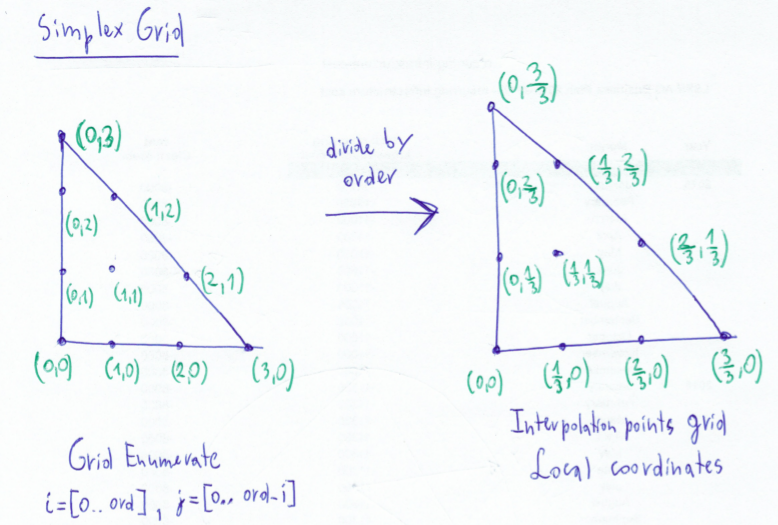
\includegraphics[scale=0.5]{doc-pics/pic-simplex-grid.png}
    %\caption{Awesome Image}
    %\label{fig:awesome_image}
\end{figure}

\noindent
After the monomials and the parametric interpolation points have been constructed, it remains to construct the interpolation matrix by evaluating the monomials at the interpolation points, then to invert the matrix, and multiply the monomial vector by it obtaining lagrange polynomials. This has been implemented both explicitly, by calculating all the lagrange interpolatory polynomials for simplices and writing them as functions, and implicitly, by introducing a polynomial class, which has all the above functionality, and thus generates a set of interpolatory polynomials which can be evaluated and integrated analytically by the code.


%%%%%%%%%%%%%%%%%%%%%%%%%%%%%%%%%%%%%%%
% Theory for global and local mappings
%%%%%%%%%%%%%%%%%%%%%%%%%%%%%%%%%%%%%%%
\section{Coordinate transformation}

\subsection{Jacobian and JacobianInverse}

From the ElementInterpolation class one can request a complete analytical interpolatory polynomial for each of the coordinates $x,y,z$. Then one uses the polynomial methods differentiate and evaluate to calculate $J_{ij} = \partial_i p_j (u,v,w) |_{u_0, v_0, w_0}$. The inverse and determinant are obtained using JacobianInverse class, which uses MatrixHelper to invert matrix and calculate the pseudodeterminant $\sqrt{\det(JJ^T)}$. \\

\subsection{Local-to-Global mapping}

The global coordinate is obtained by calling the corresponding method $realCoordinate()$ of the Interpolator class. It evaluates a linear combination of lagrange polynomials for each coordinate.

\subsection{Global-to-Local mapping}

This method finds local coordinate within this element from a given global coordinate. The $is\_inside()$ method is part of this method, as it returns false if the point is not within the element, and true + the local coordinate, if the point is. \\

\noindent
After a discussion the following was agreed on:
\begin{itemize}
	\item $local()$ method is not defined outside the element. Even for most simple polynomial maps, there exist global coordinates which do not correspond to any local coordinate at all. For example, $x^2$ is a perfectly valid local-to-global map for an edge defined on $[0,1]$, however, no local coordinate at all corresponds to the global coordinate $-1$. Therefore, if we have high evidence that a point is located outside the element, we only report that it is outside and do not report any local coordinate. As the local coordinate is found using an iterative process, it needs to have a termination condition, because, given that a local coordinate of interest does not exist, the method will not converge.
	\item $local()$ method is only defined when $(dim_{elem} = dim_{world})$. For inequal dimensions, disregarding the question being a challenging computational task, it is also meaningless. The probability that a randomly selected point would belong to a manifold of dimension lower than the world dimension is negligibly small. If the point is non-random, it must have been generated using a local-to-global map of one of the elements, in which case there are much more cost-efficient ways of tracing it back, for example, by storing the local coordinate mapped.
\end{itemize}

\noindent
Even considering the two above simplifications, this is still a very tricky problem. Since the map from local to global is polynomial, it is in principle non-invertible, at least not in terms of standard functions \\

\noindent
It can be guaranteed that the map is one-to-one within the element, otherwise the the real element geometry would be self-intersecting, which should be ensured by GMSH when selecting interpolation points. However, there are no obvious reasons why the geometry should not be self-intersecting outside the element, which means that the map need not be one-to-one outside the element. \\

\noindent
For obvious reasons we will not solve the problem directly, as searching for roots of a system of polynomial equations with several parameters is a very challenging task. Instead we minimize the two-norm \[\vec{r} = \mathrm{argmin} \{ |\vec{p}(\vec{r}) - \vec{p}_0 |^2 \}. \] We think that the problem should not have local extrema inside the element, because that is equivalent to having $\det J = 0$. However, it will most likely have local extrema outside the element (especially for higher orders). The solutions proposed:
\begin{itemize}
	\item Currently Dune uses Newton's method \[\vec{r}_{n+1} = \vec{r}_n + \mathrm{LinSolve}(J(\vec{r}_n), \vec{p}(\vec{r}_n) ). \] Since the mapping is 1-to-1 inside the element, it should definitely not have minima and maxima, not sure about extrema. Therefore Newton's method should converge to the right solution if the starting point is selected inside the element, for example its center.
	
	\item Termination condition:
		- The iterative solution should not be strongly outside the element for some iteration, if the true solution is inside. Therefore, we terminate if at any point $|\vec{p}_{CoM} - \vec{p}|_2 > 4 R_{lin}$, using the notation from $is\_inside()$ descriotion.
	
	\item This method may fail if there indeed is an extrema inside the element, and after an unlucky step it is thrown out of the element even though the correct solution is inside. Thus, if the method fails to find the point within the element and its neighbors this way, it may make sense to try several starting locations within each tetrahedron hoping to avoid the extrema.
\end{itemize}


%%%%%%%%%%%%%%%%%%%%%%%%%%%%%%%%%%%%%%%
% Theory for integration over curvilinear entities
%%%%%%%%%%%%%%%%%%%%%%%%%%%%%%%%%%%%%%%
\subsection{Integration}
\label{sec:theory:integration}

An important function of any entity is calculating its volume, integrating scalar and vector functions within it. In order to parametrize the integration domain, the integration is converted to local coordinates, namely
\[ \int f(\vec{x}) d^{\dim} x = \int f(\vec{r}) \mu(\vec{r}) d^{\dim} r \]
where $\vec{x}$ and $\vec{r}$ are global and local coordinates respectively, and the conversion function $\mu(\vec{r})$ is called the integration element. In the original \textit{dune-geometry} paradigm, geometry class itself does not perform any integration, but calculates the integration element$\mu(\vec{r})$. The user chooses and performs the integration over reference element by using, for example, one of the quadrature rules\cite{abramowitz+1970} provided by \textit{dune-geometry}. A standard numerical quadrature can written as a weighted sum
\[ \int f(\vec{r}) \mu(\vec{r}) d^{\dim} r = \sum_i f(\vec{r}_i) \mu(\vec{r}_i) w_i  \]
where the $r_i$ and $w_i$ are the quadrature points and weights. The sampling points and weights are a property of a quadrature rule used, and can be reused for all integrands given fixed domain and approximation order. More precisely, given a polynomial order $p$, one can construct a finite numerical quadrature, which will be exact for all functions, well approximated by polynomials of order $p$ and below. \\

\noindent
Numerical quadrature methods in practice are considerably faster than any other known method for domain dimensions $\dim \leq 3$ \cite{schurer2003}, but they also have disadvantages. Firstly, they are inaccurate for functions that can't be approximated by reasonable order polynomials. Secondly, numerical quadratures for non-trivial domains (e.g. simplices) have so far only been calculated only to very moderate orders (~20) \cite{zhang+2008}. Finding a numerical quadrature is equivalent to finding roots of a polynomial, which is extremely hard in more than 1 dimension. One way to overcome these difficulties is to transform the integration domain to a cuboid using a Duffy transform:

\[ \int_0^1 \int_0^{1-x} f(x,y) dx dy = \int_0^1 \int_0^1 f(x, (1-x)t ) dx dt  \]

\noindent
The advantage of the cuboid domain is that a quadrature rule can be constructed from a tensor product of 1D quadratures, thus only requiring the knowledge of 1D quadratures, which are available to a relatively high order. Quadrature rules created in this fashion have more points per order than the rules created specifically for the desired (e.g. simplex) domain. Nevertheless, they work, and they are implemented in \textit{dune-grid} up to order 61. There exist advanced methods to improve performance of quadrature integration (e.g. Sparse Grids \cite{petras2000}), but they are beyond the scope of this paper. \\

%%%\subsection{Overview of available numerical methods}
%%%
%%%\noindent
%%%Below is presented a short summary of integration method types known to us: \\
%%%
%%%\noindent
%%%\textbf{Gaussian Quadrature}: The method available in DUNE.
%%%\begin{itemize}
%%%	\item This method calculates the integral as a linear product of the integrand $f(\vec{r})$ values at specific precomputed points $\vec{r}_i$ with specific precomputed weights $w_i$, namely $I = \sum_i w_i f(\vec{r}_i)$. Thus the main advantage of this method is its computational cost, which is small for low order polynomial integrands.
%%%	\item Optimal quadrature points are only available for small dimensions. Finding such point sets for high dimension polynomials is very involved and is known to suffer from finite precision of floating point arithmetic. Alternatively, a suboptimal point distribution can be obtained from a tensor product space of 1D point distributions, whose size grows exponentially with integration dimension.
%%%	\item Gaussian Quadrature is constructed with the idea of calculating exact integrals for integrands being polynomial up to a given order. However, when integrating over a curved boundary, thte integration elemen is a square root of a polynomial, and polynomials really badly approximate square root, especially for small arguments, which can easily happen for highly curved elements. Not to mention that one, in principle, could with to integrate arbitrary (within reason) functions over the element. Thus
%%%		\subitem - Can GQ estimate integration error for non-polynomial functions?
%%%		\subitem - Can it be made hierarchical to have control over error by refinement?
%%%		\subitem - What would be the convergence rate to compare with other methods?
%%%\end{itemize}
%%%
%%%\noindent
%%%\textbf{Interpolatory adaptive refinement}: The method currently implemented in LagrangeGeometry subclass
%%%\begin{itemize}
%%%	\item - Evaluates integral over element, approximating the integrand by an interpolatory polymomials of two hierarchical orders (2 and 4 at the moment) \textbf{[IMAGE HERE]}
%%%	\item - The running integration error is approximated by the difference between the analytical integrals calculated from these two interpolatory polynomials.
%%%	\item - The higher order element is split into into sub-elements of lower order, and the integration proceeds recursively.
%%%	\item - Every time an element is split, its previous running error is subtracted from the total error, and the running errors of the sub-elements are added to the total error. Thus, the integration is terminated when total approximated error is below selected tolerance. 	
%%%		\subitem - using heap structure ordered by the approximate error of the element. This way avoids recursion, and at every iteration selects the element which has worst error, then refines it.
%%%		\subitem - When splitting, the previously calculated points are not re-calculated but hierarchically re-used by sub-elements. The sub-element only needs to be refined to a higher hierarchical order, by adding more points.
%%%	\item \textit{Possible improvement - Performance}. As the the refined element does not check if the neighboring elements are also being refined, so they both sample on the boundary twice. Does there exist a method to store/find intersection refinements faster than just compute 2nd time. Using order 4 for every new refined triangle we sample 9 new points, out of which 2 are being wasted, thus $22\%$ inefficient.
%%%\end{itemize}
%%%
%%%\noindent
%%%\textbf{Monte-Carlo integration} - according to above mentioned paper, good for dimensions 7 and above.
%%%\begin{itemize}
%%%	\item Randomly samples function over element, integral is approximated by the average over the sample
%%%	\item natural error estimate using sample standard deviation
%%%	\item Stratified Sampling: if after a set number of iterations sample error is larger than expected, then function is highly non-uniform. Split element in equal parts and continue recursively.
%%%	\item Markov Chain Monte Carlo (MCMC): Uses random walk to sample the integrand, thus concentrating the sample points where the function varies most. Can use Metropolis-Hastings to also adapt the sampling distribution.
%%%\end{itemize}
%%%
%%%\noindent
%%%\textbf{Interpolatory Spline integration} - this is just another idea...
%%%\begin{itemize}
%%%	\item Makes grid over element, cubic-interpolates all consecutive partially-overlapping segments, integrates analytically over each segment.
%%%		\subitem -tricky part 1: when interpolatory segments intersect, with what weights to take the intersecting parts
%%%		\subitem -tricky part 2: how well does this method interpolate boundaries of the element (being close to edges and faces)
%%%		\subitem -tricky part 3: how to estimate error of integration and necessary grid step?
%%%		\subitem - Any way to do the refinement or error-control?
%%%\end{itemize}


\subsubsection{Additional Concerns}

The integration in \textit{dune-curvilineargeometry} focuses on two additional questions:
\begin{itemize}
	\item Integrating polynomials of arbitrary order
	\item Integrating smooth functions with optimal polynomial order not known in advance.
\end{itemize}

\noindent
\textbf{Analytic Integration}\\
To address the first question, \textit{dune-curvilineargeometry} implements a polynomial class, which is stored as a sum of monomials of a given order. Integrals over monomials of a given order can be expressed analytically \cref{appendix-proof-simplexintegral} \\

\begin{table}[h]
\centering
\begin{tabular}{l | l}
\hline
Cuboid Integrals &
\begin{tabular}{@{}c@{}}
$ \int_0^1 x^i dx = \frac{1}{i+1} $ \\
$ \int_0^1 \int_0^1 x^i y^j dx dy = \frac{1}{(i+1)(j+1)} $ \\
$ \int_0^1 \int_0^1 \int_0^1 x^i y^j z^k dx dy dz = \frac{1}{(i+1)(j+1)(k+1)} $ \\
\end{tabular} \\ \hline
Simplex Integrals &
\begin{tabular}{@{}c@{}}
$ \int_0^1 x^i dx = \frac{1}{i+1} $ \\
$ \int_0^1 \int_0^{1-x} x^i y^j dx dy = \frac{i! j!}{(i + j + 2)!} $ \\
$ \int_0^1 \int_0^{1-x} \int_0^{1-x-y} x^i y^j z^k dx dy dz = \frac{i! j! k!}{(i + j + k + 3)!} $ \\
\end{tabular} \\
\end{tabular} \\
\end{table}

\noindent
We provide a method to integrate over a reference element in the polynomial class. It is exact and works simply by summing the analytical monomial integrals given above for all monomial summands. \\

\noindent
\textbf{Adaptive Integration}\\
In its most general form a scalar integral over an element can be written as \[\int f(\vec{r}) d^{\dim} x = \int f(\vec{r}) \mu(\vec{r}) d^{\dim} r,\] where the integration element $\mu(\vec{r})$ can most generally be written as \[\mu(\vec{r}) = \sqrt{\det(J J^T)},\] where $J$ is the Jacobian matrix. \\

\noindent
In the case of matching element and space dimension (like volume in 3D, and area in 2D), the integration element simplifies to $|\det J|$. Even though absolute value is not a polynomial function, it can be observed that $\det J$ is not allowed to change sign over the element for any sensible non-self-intersecting geometries. Even if $\det J = 0$ somewhere within the element, it would mean that a finite volume element inside reference element is mapped to a 0 volume in real space, which should be avoided by meshing tool. Therefore, in this case, $\det J$ will always have the same sign. It remains to evaluate it anywhere inside the element, and multiply by -1 if it is negative. Then the integration of scalar polynomial function over this integration element can be done exactly. \\

\noindent
In the case of mismatching dimensions (like area in 3D, and length in 2D and 3D), the expression for $\mu(\vec{r})$ can not be simplified, and therefore the integrand is a square root of a polynomial. This integral cannot be done analytically, and therefore requires a numerical method. Currently, \textit{dune-curvilineargeometry} provides a recursive integrator, which iteratively increases the quadrature order until the estimated integration error converges to a desired tolerance. This method can take several seconds if the integrand requires very high polynomial order, but for low order integrands it converges much faster.

\noindent
Still, there is definitely room for improvement. According to \cite{schurer2003} best results in low-dimensional numerical integration are achieved by adaptive quadrature of high degree, whereas Monte-Carlo methods are best for high-dimensional integrals. Thus, using an external adaptive library, for example the GSL extension from \url{http://ab-initio.mit.edu/wiki/index.php/Cubature}, could be of definite advantage. It is based on Clenshaw-Curtis quadrature, which has the advantage of being hierarchical, and thus can be refined to iteratively improve precision withouth having to sacrifice previous sample points. Another speedup could be provided by employing sparse grids \cite{petras2000} \\

%%%\subsection{Integration Element - Vector}
%%%
%%%When integrating vector functions we are mostly interested in the integrals over boundary surfaces and edges, namely $\int_{\partial V} \vec{f}(\vec{r}) \cdot \vec{n}(\vec{r}) d(\partial V)$. For an edge in 2D the following expression for the tangential and normal integration elements (up to a sign convention) can be found:
%%%\[ d\vec{l}_{\parallel} = (\partial_u p_x, \partial_u p_y)du \; \; \; \; \; d\vec{l}_{\perp} = (\partial_u p_y, -\partial_u p_x)du  \]
%%%
%%%\noindent
%%%For a vector in 3D the tangential integration element is not defined, but the normal integration element is
%%%\[ d\vec{S} = (\partial_u \vec{p} \times \partial_v \vec{p})du \; dv  \]
%%%
%%%\noindent
%%%Thus, given polynomial vector basis functions $\vec{f}$ and polynomial interpolation, the scalar (and, if necessary, vector) products $\vec{f}(u) \cdot d\vec{l}(u)$ and $\vec{f}(u,v) \cdot d\vec{S}(u,v)$ are also polynomial, and can be integrated exactly using analytic polynomial integration code.



%%%%%%%%%%%%%%%%%%%%%%%%%%%%%%%%%%%%%%%
% Theory for point location (OCTree)
%%%%%%%%%%%%%%%%%%%%%%%%%%%%%%%%%%%%%%%
\section{OCTree}
\label{theory-octree}

\subsection{Point location with respect to a plane}

Assume that a plane is given by 3 coordinates $\vec{a}, \vec{b}, \vec{c}$, and we would like to check on which side of this plane the point $\vec{p}$ is. This is uniquely given by a function
\begin{equation}
\label{equation-point-plane-test}
	ptest(\vec{a}, \vec{b}, \vec{c}, \vec{p}) = \mathrm{sgn} \{ \det (\vec{a} - \vec{p}, \vec{b} - \vec{p}, \vec{c} - \vec{p}) \}
\end{equation}
\noindent
This function takes values $1,-1$ for corresponding sides of the plane, and $0$ if the point is on the plane.

\subsection{Locating the element the given global coordinate belongs to}
\label{subsection-locating-element}

\noindent
Current convention: loop over all elements in the mesh, check if the point is inside the element using the method below. \\


\noindent
This method has $O(1)$ initialization cost, but $O(N) * ins$ query cost, which becomes wastefully slow as the number of points to locate grows. Here $ins$ is the cost of $is\_inside$ method, which has constant complexity if the query point is far away from the triangle, but requires an iterative method for nearby methods.

\noindent
There are two ways one can implement the above idea: \\
\textbf{First method:}
\begin{enumerate}
	\item Iterate over all elements, use linear $check\_inside()$
	\item For the element for which linear $check\_inside() = true$ run the nonlinear $check\_inside()$
	\item If the nonlinear $check\_inside() = false$, recursively do nonlinear $check\_inside()$ on the neighbors of the element.
\end{enumerate}
\textbf{Second method:}
\begin{enumerate}
	\item Iterate over all elements, use nonlinear $check\_inside()$
\end{enumerate}
\noindent
The first method is better, because it will on average have less runs of the iterative method, as if the point is located in a linear element, it has high probability of being located inside the nonlinear element with the same corners. \\

\noindent
An improvement would be to implement an OCTree, which will have a recursively-refined cubic mesh over the tetrahedral one, and upon initialization would place each of the tetrahedrons recursively within one or more leafs of the tree. Thus the initialization cost would be $O(N \log(N))$, and the cost of a single query $O(\log(N)) + M * inc$, where $M$ is the number of neighbors an element has. This is a considerable improvement for large number of queries. \\

\noindent
\textbf{OCTree method}:
\begin{enumerate}
	\item Construct the OCTree - grid the domain, build the hierarchical tree, place the correct element labels into each leaf
	\item For each query, locate the leaf the query point corresponds to
	\item Proceed by using one of the above methods on the element set of the leaf
\end{enumerate}

\begin{figure}[hp]
    \centering
    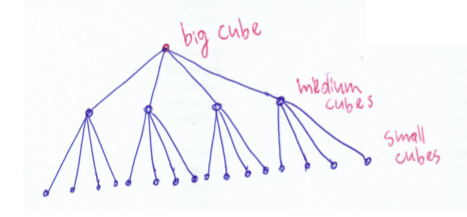
\includegraphics[scale=0.7]{doc-pics/pic-octree-3.png}
	\caption{OcTree internal structure}    
    
    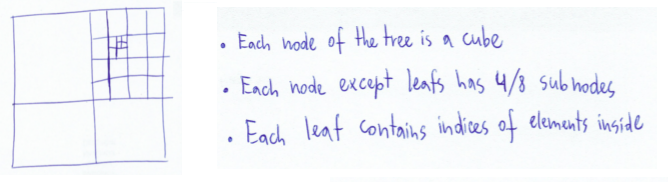
\includegraphics[scale=0.7]{doc-pics/pic-octree-1.png}
	\caption{OcTree grid}    
	
    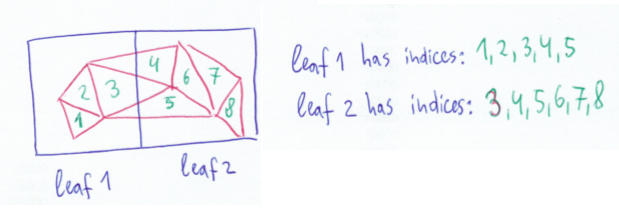
\includegraphics[scale=0.7]{doc-pics/pic-octree-2.png}
	\caption{OcTree partition of elements}    
    %\caption{Awesome Image}
    %\label{fig:awesome_image}
\end{figure}


\noindent
How does this work with parallel processing?

\subsection{Checking if a global coordinate is inside a given element (straight sided)}
\label{subsection-isinside-linear}

\noindent
For straight-sided elements the conversion between global and local coordinates is 1-to-1 in the whole space.
Therefore, it is sufficient to find the corresponding local coordinate and use the $referenceelement$ method $checkInside$. \\

\noindent
For example, for a simplex the $is\_inside(u,v,w)$ for local coordinates $(u,v,w)$ looks like 
\[u \geq 0\ \&\ v \geq 0\ \&\ w \geq 0,\ \&\ u+v+w \leq 0. \]

\noindent
Naturally, the global-local map has a finite precision, therefore the $checkInside$ method corrects for that by having a small tolerance for above inequalities, thus avoiding the case where a boundary point would be considered outside both neighboring elements because of numerical errors.


\subsection{Checking if a global coordinate is inside a given element (curvilinear elements)}
\label{subsection-isinside-nonlinear}

\noindent
This method is only defined if ($(dim_{elem} = dim_{world})$). For discussion see the $local()$ method discussion.

\noindent
In principle, this method requires an iterative solver, but first we run two simpler tests which immediately identify some of the points inside or outside of the element. \\

\noindent
\textbf{Far-point test}:
\begin{enumerate}
	\item Define linear center $\vec{p}_{CoM}$ of an element as the center of mass of its corners.
	\item Define the radius of an element $R$ as the largest distance between $\vec{p}_{CoM}$ and a point $\vec{p}_b$ on its boundary
	\item Define linear radius $R_{lin}$ to be the largest distance between $\vec{p}_{CoM}$ and one of the corners of the element. It can be shown that $R_{lin} = \frac{\sqrt{dim^2 + dim - 1}}{dim + 1} $, which is $\{ \frac{1}{2}, \frac{\sqrt{5}}{3}, \frac{\sqrt{11}}{4} \}$ for dimensions $\{1,2,3\}$.
	\item Demand that for all sensible curvilinear elements, $R$ should be bounded by some scaling of $R_{lin}$. For example, we can require that $R \leq 2 R_{lin}$, which would mean that all poins of every element should be entirely contained within $2 R_{lin}$ of its center. A more precise prefactor could be calculated from curvature constants of the bounaries of the element (max over the boundary of some expr. involving derivatives of interpolatory polynomials).
	\item Thus, if $|\vec{p}_{CoM} - \vec{p}|_2 > 2 R_{lin}$, we can immediately report that $\vec{p}$ is outside the element.
\end{enumerate}

\noindent
\textbf{Global Barycentric Coordinate test}:
\begin{enumerate}
	\item Define a global barycentric coordinate as the area enclosed by one curved boundary of the element, the point of interest, and the straight-sided boundaries that connect the point of interest and the corners of the curved boundary.
		\subitem - for 2D triangle, a barycentric coordinate is given by
		\[B = \frac{1}{2}\int_0^1 (\vec{p}(u) - \vec{p}_0) \times \partial_u \vec{p}(u) du\]
		as derived from triangle area $S = \frac{1}{2} \vec{a} \times \vec{b}$. Here $\vec{p}_0$ is the coordinate of interest.
		\subitem - for 3D tetrahedron, a barycentric coordinate is given by
		\[B = \frac{1}{3}\int_0^1 \int_0^{1-u} (\vec{p}(u,v) - \vec{p}_0) \cdot (\partial_u \vec{p}(u,v) \times \partial_v \vec{p}(u,v)) du\]
		as derived from tetrahedron volume area $V = \frac{1}{6} \vec{a} \cdot (\vec{b} \times \vec{c})$.
		Note that there is an additional factor of 2 in the barycentric equation, because triangular grid only covers half of the triangle, whereas
		parallelogram grid covers the whole (check figure \ref{fig:barycentric_coordinate_calculation})

\begin{figure}[!htb]
    \centering	
    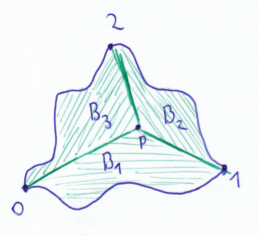
\includegraphics[scale=0.7]{doc-pics/pic-barycentric-curvilinear-definition.png}
    \caption{Definition of Barycentric Curvilinear Coordinates}
    %\label{fig:awesome_image}
\end{figure}

	\item For linear elements, the sum of barycentric coordinates always equals the total volume of the element for internal points, and is larger than that for external points. This is not true for non-convex elements, as the sum may be larger than the volume even for internal points. The method can not be improved by considering the sign of the barycentric coordinate based on the orientation of the boundary, as it is the same for internal and external points of the concave surface.
	\item Thus, if the sum of global barycentric coordinates is equal to the volume of the element, the point is automatically inside the element, otherwise we remain uncertain.
			
\end{enumerate}

\begin{figure}[!htb]
    \centering	
    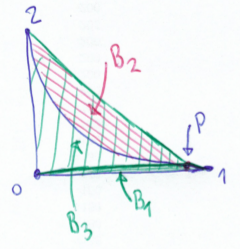
\includegraphics[scale=0.7]{doc-pics/pic-barycentric-problem-1.png}
    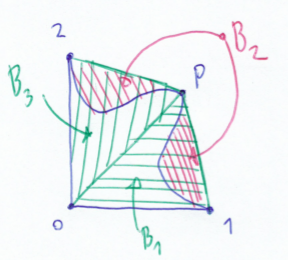
\includegraphics[scale=0.7]{doc-pics/pic-barycentric-problem-2.png}
    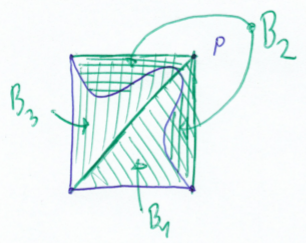
\includegraphics[scale=0.7]{doc-pics/pic-barycentric-problem-3.png}
    \caption{Problem cases with Barycentric Curvilinear coordinates}
    %\label{fig:awesome_image}
\end{figure}

\noindent
If both the above tests do not give a conclusive result, we need to use Global-To-Local mapping, and then $checkInside$ for the local coordinate. The challenges of this approach are described in the corresponding section. \\

\noindent
\textbf{Current Implementation: } There is no $is\_inside()$ method, only $local()$ method. Local method returns false if the point is not inside the element, and returns true and the correct local coordinate if it is. If the answer is true, we have to calculate the local coordinate anyway to make sure, makes sense to return it not to calculate it twice.

\begin{figure}[p]
    \centering
    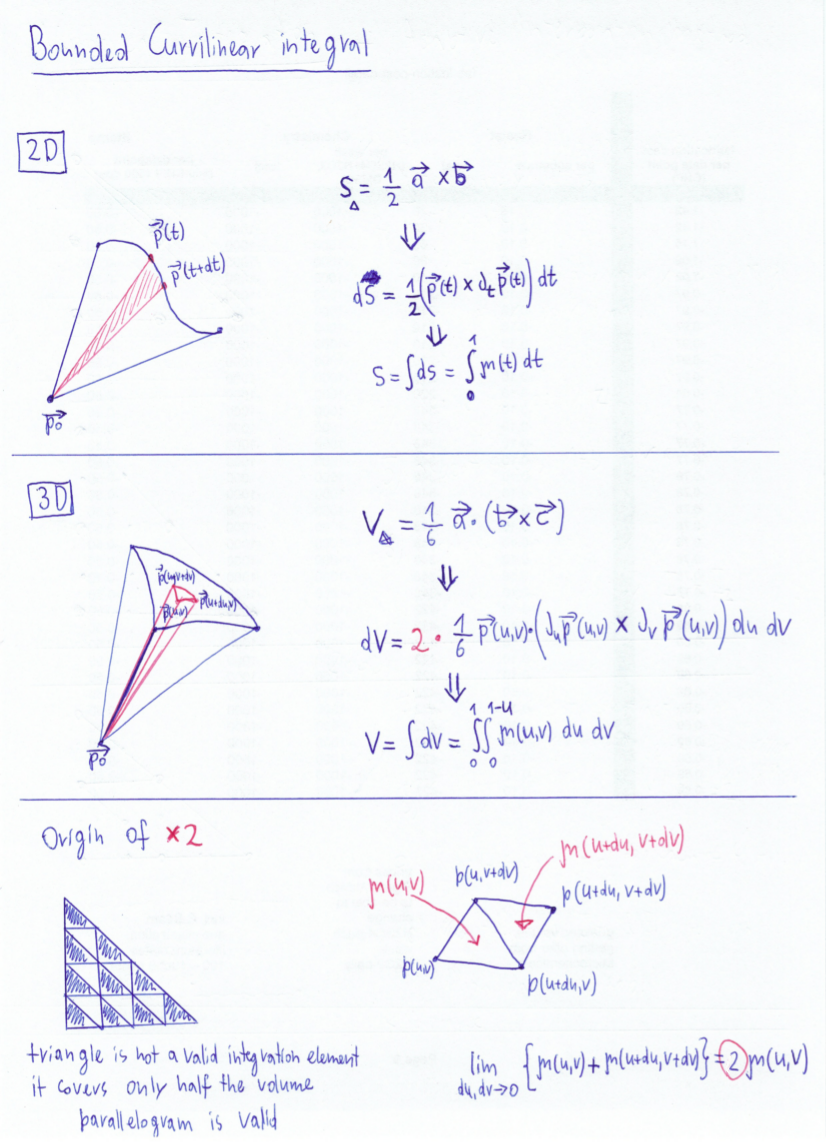
\includegraphics[scale=0.7]{doc-pics/pic-bounded-curvilinear-integral.png}
    \caption{Barycentric Coordinate Calculation}
    \label{fig:barycentric_coordinate_calculation}
\end{figure}








\chapter{Implementation Details}

%%%%%%%%%%%%%%%%%%%%%%%%%%%%%%%%%%%%%%%%%%%%%%%%%%%%%%%%%%%%%%%%%%%%%
% Implementation Details - Curvilinear Element Interpolator
%%%%%%%%%%%%%%%%%%%%%%%%%%%%%%%%%%%%%%%%%%%%%%%%%%%%%%%%%%%%%%%%%%%%%

\section{Implementation Details - Geometry}
\label{impl-geometry}

\subsection{Analytical Interpolatory Vector}
\label{impl-geometry-analytical-vector}

\noindent
Produces an analytical map from local to global coordinates in terms of polynomial vector. This implementation follows closely the section \ref{theory-lagrange}

\begin{itemize}
  \item 0) Constructs local grid points $\vec{r}_i$
  \item 1) Constructs monomial basis $\vec{z}^{ord}(\vec{r})$
  \item 2) Evaluates all monomials $\vec{z}^{ord}(\vec{r})$ at all local grid points $\vec{r}_i$, assembling the DynamicMatrix V
  \item 3) Computes all lagrange polynomials using $\vec{L}(\vec{r}) = V^{-1} \vec{z}^{ord}(\vec{r})$
  \item 4) Computes the analytical map $\vec{p}(\vec{r}) = \sum_i \vec{p}_i L_i (\vec{r})$.
\end{itemize}

\subsection{Subentity Interpolator}
\label{impl-geometry-subentity-interpolator}

\noindent
Constructs Interpolator classes for each $\dim - 1$ subentity of the given element. Only allowed for elements of dimensions 2 and 3. At the moment a rather crude algorithm is employed. To find the vertices corresponding to a given boundary, the order numbers of simplexGrid are written in a $(ord + 1) \times (ord + 1) \times (ord + 1)$ matrix, which is then used to easier locate the indices of the boundary interpolatory points in the vertex vector. Certain orientation convention is chosen for the provided sub-entitiy interpolators, to simplify the future calculation of the outwards normals. The convention for edge orientations for a triangle $(012)$ are $(01)$, $(12)$ and $(20)$. The convention for triangle orientations for a tetrahedron $(0123)$ are $(012)$, $(023)$, $(213)$ and $(031)$.


\begin{figure}[hp]
    \centering
    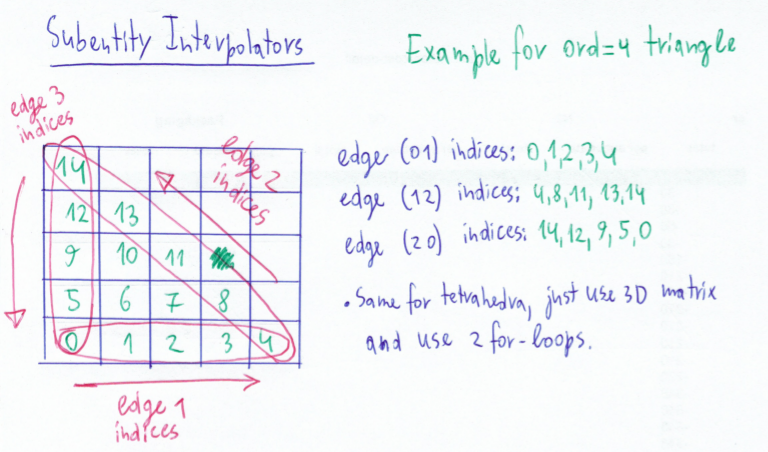
\includegraphics[scale=0.5]{doc-pics/pic-subentity-interpolators-method.png}
    %\caption{Awesome Image}
    %\label{fig:awesome_image}
\end{figure}


%%%%%%%%%%%%%%%%%%%%%%%%%%%%%%%%%%%%%%%%%%%%%%%%%%%%%%%%%%%%%%%%%%%%%
% Implementation Details - Curvilinear Geometry
%%%%%%%%%%%%%%%%%%%%%%%%%%%%%%%%%%%%%%%%%%%%%%%%%%%%%%%%%%%%%%%%%%%%%

\section{Implementation Details - Curvilinear Geometry}

\subsection{Local-to-global Mapping}

\subsection{Normals}

\subsection{Analytical Integration}


%%%%%%%%%%%%%%%%%%%%%%%%%%%%%%%%%%%%%%%%%%%%%%%%%%%%%%%%%%%%%%%%%%%%%
% Implementation Details - Curvilinear GMSH Reader
%%%%%%%%%%%%%%%%%%%%%%%%%%%%%%%%%%%%%%%%%%%%%%%%%%%%%%%%%%%%%%%%%%%%%


\section{Implementation Details - Curvilinear GMSH Reader}

\subsection{Structure of .msh files}

\begin{mybox}
\begin{lstlisting}
$MeshFormat
ver f_type data_size    # This line is mostly irrelevant
$EndMeshFormat
$Nodes
n_vertices
1 x y z
2 x y z
.......
n_vertices x y z
$EndNodes
$Elements
n_elem
1 elem_type n_tags (process_tags) v_1 v_2 ... v_N
2 elem_type n_tags (process_tags) v_1 v_2 ... v_N
.......
n_elem elem_type n_tags (process_tags) v_1 v_2 ... v_N
$EndElements
\end{lstlisting}
\end{mybox}

\noindent
where
\begin{itemize}
	\item $ver$             - version of the GMSH file
	\item $f\_type$          - type of file (irrelevant)
	\item $data\_size$       - size of file (irrelevant)
	\item $n\_vertices$      - number of vertices of the mesh
	\item $i\ x\ y\ z$         - index of the vertex and its coordinates
	\item $n\_elem$          - number of elements of the mesh
	\item $elem\_type$       - Integer which determines element type and interpolation order
	\item $n\_tags$          - Total number of tags. If $>2$, then have $process\_tags$
	\item $process\_tags$    - Tags which determine the process the vertex belongs to. Only if GMSH is told to partition the mesh
	\item $v\_1\ v\_2\ ...\ v\_N$ - Indices of interpolatory vertices associated with this element (includes corners)
\end{itemize}

\subsection{Convention for numbering interpolatory vertices}

\noindent
Each curvilinear element posesses a set of interpolatory vertices. For order 1 (linear elements) this is just the set of corners of the element, but for higher orders there are additional points located in on the inside of the elements, their faces and edges. To number these vertices, GMSH uses recursive conviention.

\begin{enumerate}
	\item First number all corners, then all edges, then all faces, then vertices inside element, then internal vertices of the element
	\item Inside edge, vertices are numbered sequentially
	\item For a triangle, the order of edges is $(0,1)$, $(1,2)$, $(2,0)$. (in 2D)
	\item For a tetrahedron, the order of edges is $(0,1)$, $(1,2)$, $(2,0)$, $(3,0)$, $(3,2)$, $(3,1)$.
	\item For a tetrahedron, the order of faces is $(0, 2, 1)$, $(0, 1, 3)$, $(0, 3, 2)$, $(3, 1, 2)$, including orientation
	\item If there are vertices associated with element itself(for example, on the triangle or inside the tetrahedron), a smaller element is created inside this triangle preserving its orientation, and is then numbered recursively.
\end{enumerate}

\noindent
Unfortunately, this convention does not match the grid convention used in DUNE, namely
\begin{mybox}
\begin{lstlisting}
for (z=0 to 1, y=0 to 1-z, x=0 to 1-z-y) { vertex(x,y,z); }
\end{lstlisting}
\end{mybox}

\noindent
There is no good expression which maps from GMSH to DUNE convention, so it was implemented it by hand for simplex geometries up to order 5.
\begin{itemize}
	\item Triangle Order 1: \{0, 1, 2\}
	\item Triangle Order 2: \{0, 3, 1, 5, 4, 2\}
	\item Triangle Order 3: \{0, 3, 4, 1, 8, 9, 5, 7, 6, 2\}
	\item Triangle Order 4: \{0, 3, 4, 5, 1, 11, 12, 13, 6, 10, 14, 7, 9, 8, 2\}
	\item Triangle Order 5: \{0, 3, 4, 5, 6, 1, 14, 15, 18, 16, 7, 13, 20, 19, 8, 12, 17, 9, 11, 10, 2\}
	
	\item Tetrahedron Order 1: \{0, 3, 1, 2\}
	\item Tetrahedron Order 2: \{0, 7, 3, 4, 9, 1, 6, 8, 5, 2\}
	\item Tetrahedron Order 3: \{0, 11, 10, 3, 4, 17, 14, 5, 15, 1, 9, 18, 12, 16, 19, 6, 8, 13, 7, 2\}
	\item Tetrahedron Order 4: \{0, 15, 14, 13, 3, 4, 25, 27, 19, 5, 26, 20, 6, 21, 1, 12, 28, 29, 16, 22, 34, 31, 24, 32, 7, 11, 30, 17, 23, 33, 8, 10, 18, 9, 2\}
	\item Tetrahedron Order 5: \{0, 19, 18, 17, 16, 3, 4, 34, 39, 36, 24, 5, 37, 38, 25, 6, 35, 26, 7, 27, 1, 15, 40, 43, 41, 20, 28, 52, 55, 46, 33, 53, 49, 30, 47, 8, 14, 45, 44, 21, 31, 54, 51, 32, 50, 9, 13, 42, 22, 29, 48, 10, 12, 23, 11, 2\}
\end{itemize}


\subsection{Parallel Implementation}

The idea of parallel implementation is that all data - vertex coordinates, internal elements and boundary elements - are split between processes, not to exceed the single core memory. Thus the strategy for reading data on a process $i$ is as follows:
\begin{enumerate}
	\item Compute the total number $N_{elem}$ of non-boundary (internal) elements.
\end{enumerate}

\begin{mybox}
Loop over all elements in the file, and count the number of elements with dimension equal to the world dimension
\end{mybox}	
\begin{enumerate}[resume]	
	\item Read and store internal elements belonging to this process. If elements are split in consequent equal chunks among processes, then process $rank$ should read the elements with indices $interv(rank) = \floor[\Big]{ [rank, rank+1] \cdot N_{elem} / p_{tot} } + 1$.
\end{enumerate}

\begin{mybox}
\begin{itemize}
	\item Loop over all elements in the file
	\item Store all internal elements for which $index \in interv(rank)$
	\item Add global indices of vertices belonging to selected elements to a set
\end{itemize}

\end{mybox}		


\begin{enumerate}[resume]
	\item Read and store boundary elements belonging to this process - those which match the subentities of some elements.
\end{enumerate}
\begin{mybox}
	\begin{itemize}
		\item Only read the boundaries for which all \textbf{corners} have already been included to the element vertex set. 
	\end{itemize}
\end{mybox}	

\begin{enumerate}[resume]
	\item Read and store vertices belonging to this process. Namely, all the vertices that are necessary to construct the elements and boundaries belonging to 
this process.
	\begin{itemize}
		\item Local index of a vertex is a number $[0,n_p)$ where $n_p$ is the total number of vertices on the process.
		\item Local index of a vertex is given by the order they are inserted to the grid factory. It is in the ascending order of the global index, just that certain vertices of global index are not on this process. To keep track of this we fill the global-to-local map for vertices.
	\end{itemize}

	\item Add boundary elements to factory. It is necessary to connect the boundary elements to the internal elements they share a face with, because during load balance, the boundaries need to be communicated together with the corresponding elements.GMSH does not provide information on this interconnection.
	\begin{itemize}
		\item \uline{Important!} This must be done before adding internal elements to factory, as we also need to add the interconnection array.
		\item Add global element index as well
	\end{itemize}
\end{enumerate}

\begin{mybox}
\noindent
Currently using brute-force, because it is not much slower than improved for \\

\noindent
\uline{Trivial Algorithm: (Complexity $O(12 N_{elem} N_{\beta} / p_{tot}^2)$)}\\
\textit{Loop over all stored boundary elements $\beta_i$, and over all stored internal elements $E_j$.} \\
\textit{ If $\beta_i \in E_j$ for some $j$ then store $\beta_i$ }\\

\noindent
\uline{Improved Algorithm: (Complexity $O(12 N_{elem} \log_2 (N_{\beta} / p_{tot}) / p_{tot}$)}\\

\begin{enumerate}
	\item Construct map from boundary vertex index set to boundary id
	\item Add all boundaries to the map
	\item Loop over each face of all internal elements
	\begin{enumerate}
		\item If $map[face]$ is non-null, link the element and boundary
	\end{enumerate}
\end{enumerate}

\end{mybox}	
		
\begin{enumerate}[resume]
	\item Add internal elements to factory
\end{enumerate}
\begin{mybox}
	\begin{itemize}
		\item For debugging purposes write each element to a .vtk file using CurvilinearVTKWriter.
		\item Add element vertices and global element index to factory
		\item If creating grid with boundaries, also pass $internal\_to\_boundary\_element\_linker$. This array stores the indices of boundaries which are connected to this element (if any).
	\end{itemize}
\end{mybox}







\subsection{Partitioning}


%%%%%%%%%%%%%%%%%%%%%%%%%%%%%%%%%%%%%%%%%%%%%%%%%%%%%%%%%%%%%%%%%%%%%
% Implementation Details - Curvilinear Grid Constructor
%%%%%%%%%%%%%%%%%%%%%%%%%%%%%%%%%%%%%%%%%%%%%%%%%%%%%%%%%%%%%%%%%%%%%

\section{Implementation Details - Grid Constructor}
\subsection{Global index construction}
\subsection{Ghost element construction}
\subsection{Communication interface construction}


%%%%%%%%%%%%%%%%%%%%%%%%%%%%%%%%%%%%%%%%%%%%%%%%%%%%%%%%%%%%%%%%%%%%%
% Implementation Details - Curvilinear VTK Writer
%%%%%%%%%%%%%%%%%%%%%%%%%%%%%%%%%%%%%%%%%%%%%%%%%%%%%%%%%%%%%%%%%%%%%

\section{Implementation Details - Curvilinear VTK Writer}

\subsection{Implementation}

\begin{enumerate}
  \item For each tetrahedron, define interpolation class, which gives its global curved coordinates based on local parametric coordinates and interpolation points.
      \subitem - the interpolation points are passed only once when initialising the class
  \item parametrically Loop over all surfaces of the tetrahedron
      \subitem - Shrink the surfaces by a little bit for better visibility
      \subitem - Calculate a fixed number of equally spaced points on each face using square mesh, add all points to a map, which notes which points have already been added. This can be done either by using the interpolation class to get the interpolated points, or simply re-using the interpolation points not to invoke the interpolation process at all thus testing it.
      \subitem - Split each square into 2 triangles and add them to the triangle list. If the square is at the edge, it produces only 1 triangle.
  \item Write a .VTK file which has all triangles
\end{enumerate}


\subsection{Optimal Sampling Rate}

Here we would like to discuss how many sampling points are required to represent the bounded curve using linear interpolation. This is necessary, for example, for visualisation. For a line segment, interpolating the curve bounded by 2 points, the analytic error is bounded by
\begin{equation}
	\epsilon = |f(x) - g(x)| \leq \frac{1}{8} \max_{z \in [x_a, x_b]} \{ g''(z)  \} (x_a - x_b)^2
\end{equation}
\noindent
where $f(x)$ is the line segment, $g(x)$ is the original function. $x_a$ and $x_b$ are arguments of the endpoints of the interval. \\

\noindent
Given a large interval $L$ which we split into $N$ equal segments such that $x_b - x_a = L/N$, the maximal error over all interpolated intervals is bounded by
\begin{equation}
	\epsilon_{\max} \leq \frac{L^2}{8 N^2} \max_{z \in L} \{ g''(z) \}
\end{equation}
\noindent
This can be rewritten to obtain the necessary interval number per edge
\begin{equation}
	N = \biggl \lceil \alpha \sqrt{ \max_{z \in L} \{ g''(z) \} } \biggr \rceil
\end{equation}
\noindent
where $\alpha$ depends on precision and length of the interval. We observe that there is a problem with this formula, namely that if $g''(z) = 0$ we get 0 intervals, and if $g''(z)$ is small, we get 1 interval, and we would like 2, because there is at least some curvature, and it should be emphasized that the case is different from just straight line. Therefore we empirically modify the formula
\begin{equation}
	N = \biggl \lceil \alpha \sqrt{ \max_{z \in L} \{ g''(z) \} } + 1 \biggr \rceil
\end{equation}

\noindent
Finally, since this equation is not exactly accurate for surfaces, and it is rather hard to make sense of optimal relative error, it is much easier to choose $\alpha$ empirically. We will generally operate with unit length edges ($L = 1$), and would like to, for example, have 5 points per edge with standard quadratic curvature $g(x) = x^2$. We obtain that $\alpha \approx 2.8$. \\

\noindent
As a rule of thumb, we can calculate the expected number of intervals for a standard function $g(x) = \sum_i x^i$ using this formula. The first 5 orders will produce edge intervals $\{ 1, 5, 9, 17, 35\}$, which will correspond to the number of vertices per edge $\{ 2, 6, 10, 18, 36\}$, and thus the number of surface vertices ($i(i+1)/2$) will be given by $\{3, 21, 55, 171, 666\}$.







\appendix

\chapter{Proofs}

%%%%%%%%%%%%%%%%%%%%%%%%%%%%%%%%%%%%%%%
% Proof of polynomial integral over simplex
%%%%%%%%%%%%%%%%%%%%%%%%%%%%%%%%%%%%%%%
\section{Proof for polynomial summand integrals}
\label{appendix-proof-simplexintegral}


\noindent
Note that the series for beta-function can be written as
\[B(a+1,b+1) = \int_0^1 x^a (1-x)^b dx = \int_0^1 x^a \sum_{i=0}^b C_b^i (-1)^i x^i = \sum_{i=0}^b \frac{(-1)^i C_b^i}{a+1+i}\]

\noindent
where $C_b^i = \frac{b!}{i!(b-i)!}$ is the combinations number. \\

\noindent
\textbf{1D:} \\

\begin{equation}
	I_{1D} = \int_0^1 x^{\alpha} dx = \frac{x^{a + 1}}{a + 1} \biggr |_0^1 = \frac{1}{a + 1}
\end{equation}

\noindent
\textbf{2D:} \\

\begin{eqnarray*}
	I_{2D} = \int_0^1 \int_0^{1-x} x^{a} y^{b} dx dy
	& = & \frac{1}{b+1} \int_0^1 x^{a} (1-x)^{b+1} dx = \frac{1}{b+1} \beta(a + 1, b + 2) \\
	& = & \frac{1}{b+1} \frac{a!(b+1)!}{(a+b+2)!} = \frac{a!b!}{(a+b+2)!}
\end{eqnarray*}

\noindent
\textbf{3D:} \\

\begin{eqnarray*}
	I_{3D}
	& = & \int_0^1 \int_0^{1-x} \int_0^{1-x-y} x^a y^b z^c dx dy dz \\
	& = & \frac{1}{c+1} \int_0^1 \int_0^{1-x} x^a y^b (1-x-y)^{c+1} dx dy \\
	& = & \frac{1}{c+1} \int_0^1 \int_0^{1-x} x^a y^b \sum_{i=0}^{c+1} C_{c+1}^i (-1)^i y^i (1-x)^{c+1-i} dx dy \\
	& = & \sum_{i=0}^{c+1} \frac{C_{c+1}^i (-1)^i}{c+1} \int_0^1 \ x^a (1-x)^{c+1-i} \int_0^{1-x} y^{b+i} dx dy \\
	& = & \sum_{i=0}^{c+1} \frac{C_{c+1}^i (-1)^i}{(c+1)(b+1+i)} \int_0^1 \ x^a (1-x)^{c+1-i} (1-x)^{b+1+i} dx \\
	& = & \sum_{i=0}^{c+1} \frac{C_{c+1}^i (-1)^i}{(c+1)(b+1+i)} \int_0^1 \ x^a (1-x)^{b+c+2} dx \\
	& = & \sum_{i=0}^{c+1} \frac{C_{c+1}^i (-1)^i}{(c+1)(b+1+i)} \beta(a+1, b+c+3) \\
	& = & \frac{1}{c+1} \beta(b+1,c+2) \beta(a+1, b+c+3) \\
	& = & \frac{1}{c+1} \frac{b!(c+1)!}{(b+c+2)!} \frac{a! (b+c+2)!}{(a+b+c+3)!} \\
	& = &  \frac{a! b! c!}{(a+b+c+3)!}
\end{eqnarray*}









%%%%%%%%%%%%%%%%%%%%%%%%%%%%%%%%%%%%%%%
% Bibliography
%%%%%%%%%%%%%%%%%%%%%%%%%%%%%%%%%%%%%%%


%\bibliographystyle{plainnat}
%\bibliography{oswald,numerical_libraries,molecular_plasmonics,finite_element_method,electromagnetic}


\printindex

\end{document}